%% abtex2-modelo-trabalho-academico.tex, v-1.9.2 laurocesar
%% Copyright 2012-2014 by abnTeX2 group at http://abntex2.googlecode.com/
%%
%% This work may be distributed and/or modified under the
%% conditions of the LaTeX Project Public License, either version 1.3
%% of this license or (at your option) any later version
%% The latest version of this license is in
%%   http://www.latex-project.org/lppl.txt
%% and version 1.3 or later is part of all distributions of LaTeX
%% version 2005/12/01 or later.
%%
%% This work has the LPPL maintenance status `maintained'.
%%
%% The Current Maintainer of this work is the abnTeX2 team, led
%% by Lauro César Araujo. Further information are available on
%% http://abntex2.googlecode.com/
%%
%% This work consists of the files abntex2-modelo-trabalho-academico.tex,
%% abntex2-modelo-include-comandos and abntex2-modelo-references.bib
%%

% ------------------------------------------------------------------------
% ------------------------------------------------------------------------
% abnTeX2: Modelo de Trabalho Academico (tese de doutorado, dissertacao de
% mestrado e trabalhos monograficos em geral) em conformidade com
% ABNT NBR 14724:2011: Informacao e documentacao - Trabalhos academicos -
% Apresentacao
% ------------------------------------------------------------------------
% ------------------------------------------------------------------------

\documentclass[
  % -- opções da classe memoir --
  12pt,       % tamanho da fonte
  openright,      % capítulos começam em pág ímpar (insere página vazia caso preciso)
  oneside,      % para impressão em verso e anverso. Oposto a oneside
  a4paper,      % tamanho do papel.
  % -- opções da classe abntex2 --
  %chapter=TITLE,   % títulos de capítulos convertidos em letras maiúsculas
  %section=TITLE,   % títulos de seções convertidos em letras maiúsculas
  %subsection=TITLE,  % títulos de subseções convertidos em letras maiúsculas
  %subsubsection=TITLE,% títulos de subsubseções convertidos em letras maiúsculas
  % -- opções do pacote babel --
  english,      % idioma adicional para hifenização
  french,        % idioma adicional para hifenização
  spanish,     % idioma adicional para hifenização
  brazil        % o último idioma é o principal do documento
  ]{abntex2-decsi}

% ---
% Pacotes básicos
% ---
\usepackage{enumitem}
\usepackage{lmodern}      % Usa a fonte Latin Modern
\usepackage[T1]{fontenc}    % Selecao de codigos de fonte.
\usepackage[utf8]{inputenc}   % Codificacao do documento (conversão automática dos acentos)
\usepackage{lastpage}     % Usado pela Ficha catalográfica
\usepackage{indentfirst}    % Indenta o primeiro parágrafo de cada seção.
\usepackage{color}        % Controle das cores
\usepackage{graphicx}     % Inclusão de gráficos
\usepackage{microtype}    % para melhorias de justificação
\usepackage{float}
\usepackage{caption}
\usepackage{subcaption}
% ---

% ---
% Pacotes adicionais, usados apenas no âmbito do Modelo Canônico do abnteX2
% ---
\usepackage{lipsum}       % para geração de dummy text
\usepackage[geometry]{ifsym}
\usepackage{multicol}
\usepackage{pdfpages}
% ---

% ---
% Pacotes de citações
% ---
\usepackage[brazilian,hyperpageref]{backref}   % Paginas com as citações na bibl
\usepackage[alf]{abntex2cite} % Citações padrão ABNT

% FBO: Review
\usepackage{color}
\newcommand{\review}[1]{{\textbf{\color{red}{#1}}}}

% FBO: Sugestões/questionamentos gerais:

% - O modelo é aprovado pelo COSI? Fiz tudo que o Elton tinha pedido, acredito que esteja correto. A resolução pedi para seguir o modelo do site da SISBIN, mas o site está em atualização
% - Termos em inglês -> itálico (pronto)
% - Lista de símbolos? Tinha no modelo da ABNTEX por isso eu inclui. Eu vou comentar se não precisar
% - Substitur termos:
% 	= forma -> modo, maneira (pronto)
% 	= 

% ---
% CONFIGURAÇÕES DE PACOTES
% ---

% ---
% Configurações do pacote backref
% Usado sem a opção hyperpageref de backref
\renewcommand{\backrefpagesname}{Citado na(s) página(s):~}
% Texto padrão antes do número das páginas
\renewcommand{\backref}{}
% Define os textos da citação
\renewcommand*{\backrefalt}[4]{
  \ifcase #1 %
    Nenhuma citação no texto.%
  \or
    Citado na página #2.%
  \else
    Citado #1 vezes nas páginas #2.%
  \fi}%
% ---

% ---
% Informações de dados para CAPA e FOLHA DE ROSTO
% ---
\titulo{Desenvolvimento de um Sistema Web para Controle de Faltas da Universidade Federal de Ouro Preto}
\autor{Bárbara Chesman Almeida}
\local{João Monlevade}
\dia{30}
\mes{8}
\ano{2017} % Indicar apenas o ano da monografia


% ---
% Dados da Universidade e Curso
% ---
\instituicao{Universidade Federal de Ouro Preto}
\instituto{Instituto de Ciências Exatas e Aplicadas}
\departamento{Departamento de Computação e Sistemas}
\colegiado{Colegiado de Sistemas de Informação}
%\colegiado{Colegiado de Engenharia de Computação}
\curso{Sistemas de Informação}
%\curso{Engenharia de Computação}
\grau{Bacharel em Sistemas de Informação}
%\disciplina{CEA499 - Trabalho de Conclusão de Curso II}
%\disciplina{CEA499 - Trabalho de Conclusão de Curso II}

% ---
% Dados de Orientação e Banca de Defesa
% ---
\orientador{Prof Dr. Fernando Bernardes de Oliveira}
\orientadorTitulacao{Mestre/Doutor em Ciência da Computação}
\orientadorDepartamento{DECSI - Universidade Federal de Ouro Preto}

\coorientador{Mestrando João Pedro Moura}
\coorientadorTitulacao{Mestre/Doutor em }
\coorientadorDepartamento{DECSI - Universidade Federal de Ouro Preto}

\convidadoUm{Nome Completo Convidado1}
\convidadoUmTitulacao{Doutor em Engenharia Elétrica}
\convidadoUmDepartamento{DECSI - UFOP}

\convidadoDois{Nome Completo Convidado2}
\convidadoDoisTitulacao{Doutor em Engenharia de Produção}
\convidadoDoisDepartamento{DEENP - UFOP}

% Tamanho da linha de assinatura segundo o tamanho do maior nome
% Sugestão: 8cm
\setlength{\ABNTEXsignwidth}{10cm}

% ---
% Tipo de Trabalho
% ---
\tipotrabalho{Monografia (graduação)}

% ---
% Configurações de aparência do PDF final

% alterando o aspecto da cor azul
\definecolor{blue}{RGB}{41,5,195}

% informações do PDF
\makeatletter
\hypersetup{
      %pagebackref=true,
    pdftitle={\@title},
    pdfauthor={\@author},
      pdfsubject={\imprimirpreambulo},
      pdfcreator={LaTeX with abnTeX2},
    pdfkeywords={abnt}{latex}{abntex}{abntex2}{trabalho acadêmico},
    colorlinks=true,          % false: boxed links; true: colored links
      linkcolor=blue,           % color of internal links
      citecolor=blue,           % color of links to bibliography
      filecolor=magenta,          % color of file links
    urlcolor=blue,
    bookmarksdepth=4
}
\makeatother
% ---

% ---
% Espaçamentos entre linhas e parágrafos
% ---

% O tamanho do parágrafo é dado por:
\setlength{\parindent}{1.3cm}

% Controle do espaçamento entre um parágrafo e outro:
\setlength{\parskip}{0.2cm}  % tente também \onelineskip

% ---
% compila o indice
% ---
\makeindex
% ---

% ----
% Início do documento
% ----
\begin{document}

% Retira espaço extra obsoleto entre as frases.
\frenchspacing

% ----------------------------------------------------------
% ELEMENTOS PRÉ-TEXTUAIS
% ----------------------------------------------------------
% \pretextual

% ---
% Capa
% ---
\imprimircapa
% ---

% ---
% Folha de rosto
% (o * indica que haverá a ficha bibliográfica)
% ---
\imprimirfolhaderosto*
% ---

% ---
% Inserir a ficha bibliografica
% ---

% Isto é um exemplo de Ficha Catalográfica, ou ``Dados internacionais de
% catalogação-na-publicação''. Você pode utilizar este modelo como referência.
% Porém, provavelmente a biblioteca da sua universidade lhe fornecerá um PDF
% com a ficha catalográfica definitiva após a defesa do trabalho. Quando estiver
% com o documento, salve-o como PDF no diretório do seu projeto e substitua todo
% o conteúdo de implementação deste arquivo pelo comando abaixo:
%
% \begin{fichacatalografica}
%     \includepdf{fig_ficha_catalografica.pdf}
% \end{fichacatalografica}

% \begin{fichacatalografica}
%   \vspace*{\fill}         % Posição vertical
%   \hrule              % Linha horizontal
%   \begin{center}          % Minipage Centralizado
%   \begin{minipage}[c]{12.5cm}   % Largura

%   \imprimirautor

%   \hspace{0.5cm} \imprimirtitulo  / \imprimirautor. --
%   \imprimirlocal, \imprimirdatadedefesa-

%   \hspace{0.5cm} \pageref{LastPage} p. : il. (algumas color.) ; 30 cm.\\

%   \hspace{0.5cm} \imprimirorientadorRotulo~\imprimirorientador\\

%   \hspace{0.5cm}
%   \parbox[t]{\textwidth}{\imprimirtipotrabalho~--~\imprimirinstituicao,
%   \imprimirdatadedefesa.}\\

%   \hspace{0.5cm}
%     1. Palavra-chave1.
%     2. Palavra-chave2.
%     I. Orientador.
%     II. Universidade xxx.
%     III. Faculdade de xxx.
%     IV. Título\\

%   \hspace{8.75cm} CDU 02:141:005.7\\

%   \end{minipage}
%   \end{center}
%   \hrule
% \end{fichacatalografica}

% ---

% ---
% Inserir errata
% ---
% \begin{errata}
% Elemento opcional da \citeonline[4.2.1.2]{NBR14724:2011}. Exemplo:

% \vspace{\onelineskip}

% FERRIGNO, C. R. A. \textbf{Tratamento de neoplasias ósseas apendiculares com
% reimplantação de enxerto ósseo autólogo autoclavado associado ao plasma
% rico em plaquetas}: estudo crítico na cirurgia de preservação de membro em
% cães. 2011. 128 f. Tese (Livre-Docência) - Faculdade de Medicina Veterinária e
% Zootecnia, Universidade de São Paulo, São Paulo, 2011.

% \begin{table}[htb]
% \center
% \footnotesize
% \begin{tabular}{|p{1.4cm}|p{1cm}|p{3cm}|p{3cm}|}
%   \hline
%    \textbf{Folha} & \textbf{Linha}  & \textbf{Onde se lê}  & \textbf{Leia-se}  \\
%     \hline
%     1 & 10 & auto-conclavo & autoconclavo\\
%    \hline
% \end{tabular}
% \end{table}

% \end{errata}
% ---

% ---
% Inserir folha de aprovação
% ---

% Isto é um exemplo de Folha de aprovação, elemento obrigatório da NBR
% 14724/2011 (seção 4.2.1.3). Você pode utilizar este modelo até a aprovação
% do trabalho. Após isso, substitua todo o conteúdo deste arquivo por uma
% imagem da página assinada pela banca com o comando abaixo:
%
% \includepdf{folhadeaprovacao_final.pdf}
%

% \imprimirfolhadeaprovacao
% ---

% ---
% Dedicatória
% ---
% \begin{dedicatoria}
%    \vspace*{\fill}
%    \centering
%    \noindent
%    \textit{ Este trabalho é dedicado às crianças adultas que,\\
%    quando pequenas, sonharam em se tornar cientistas.} \vspace*{\fill}
% \end{dedicatoria}
% ---

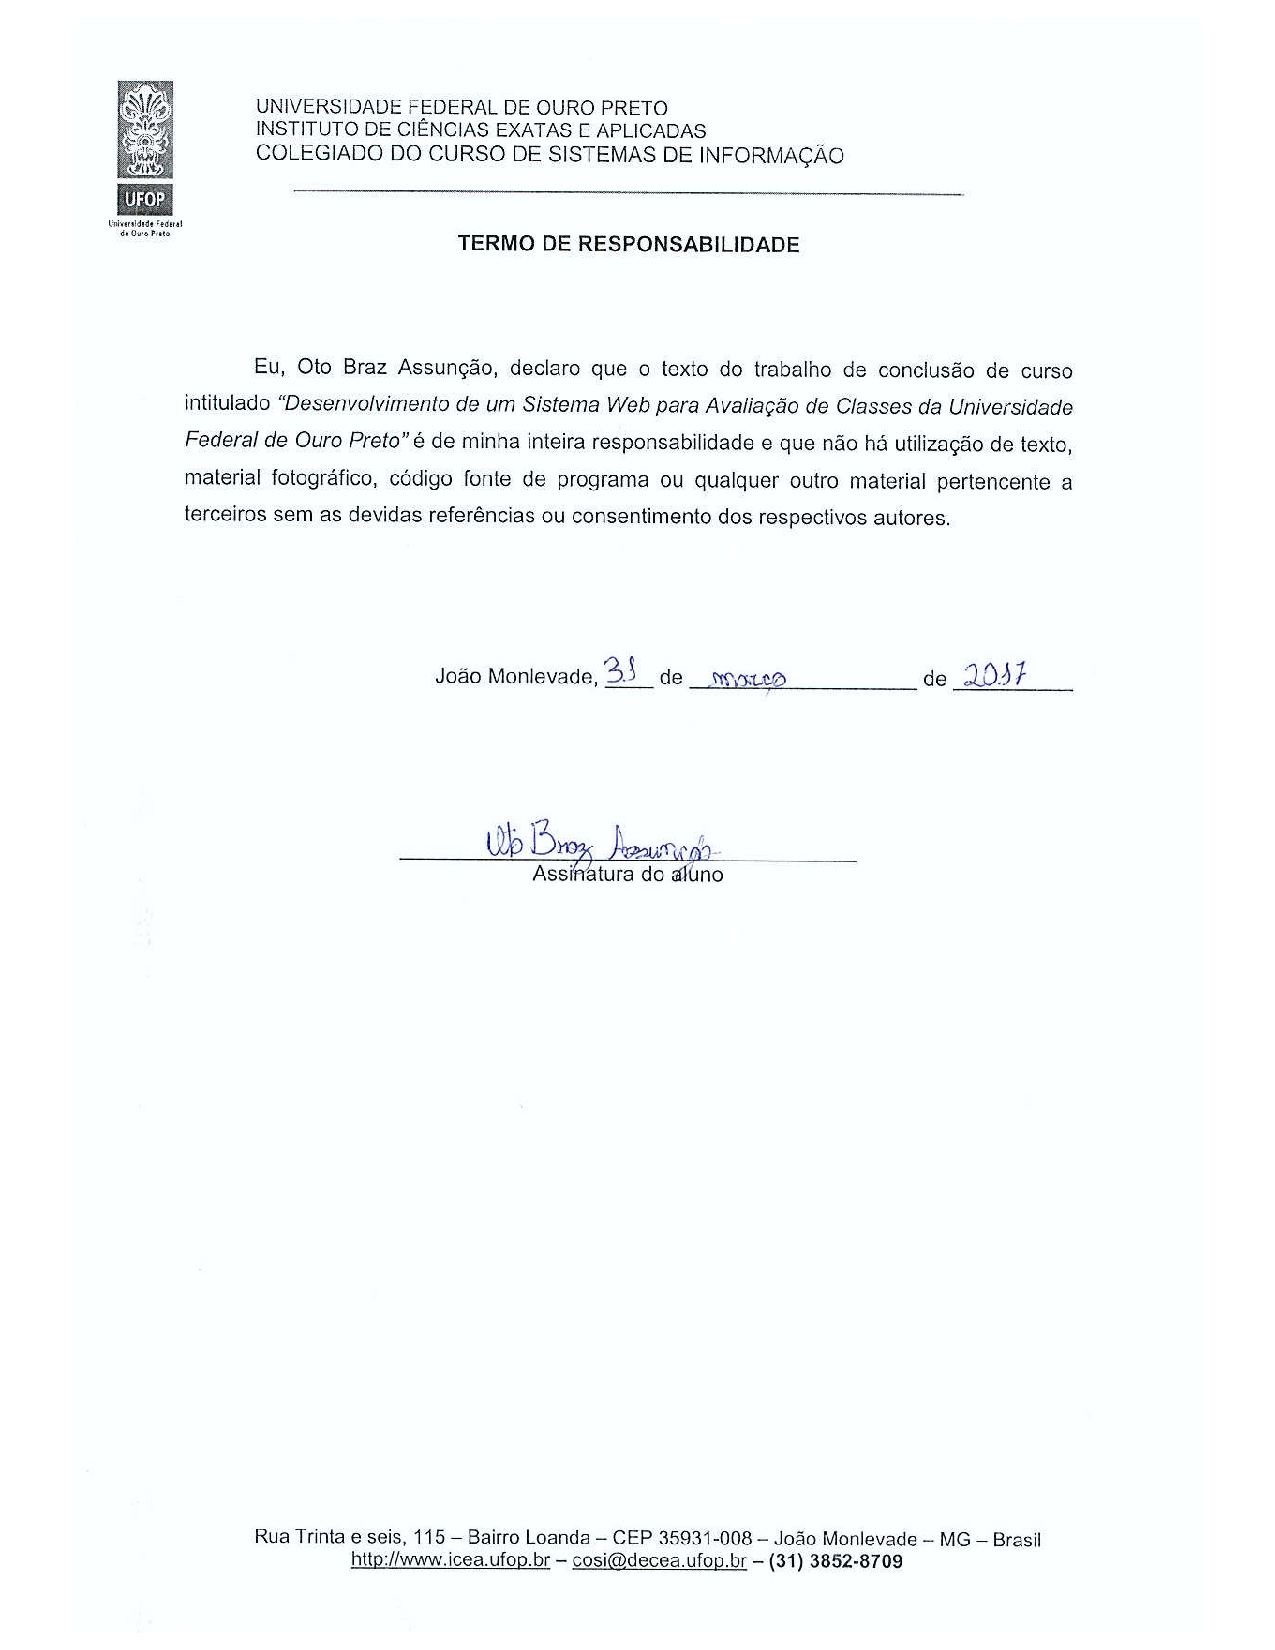
\includepdf{termoresponsibilidade.pdf}

% 
\includepdf{folhaaprovacao.pdf}

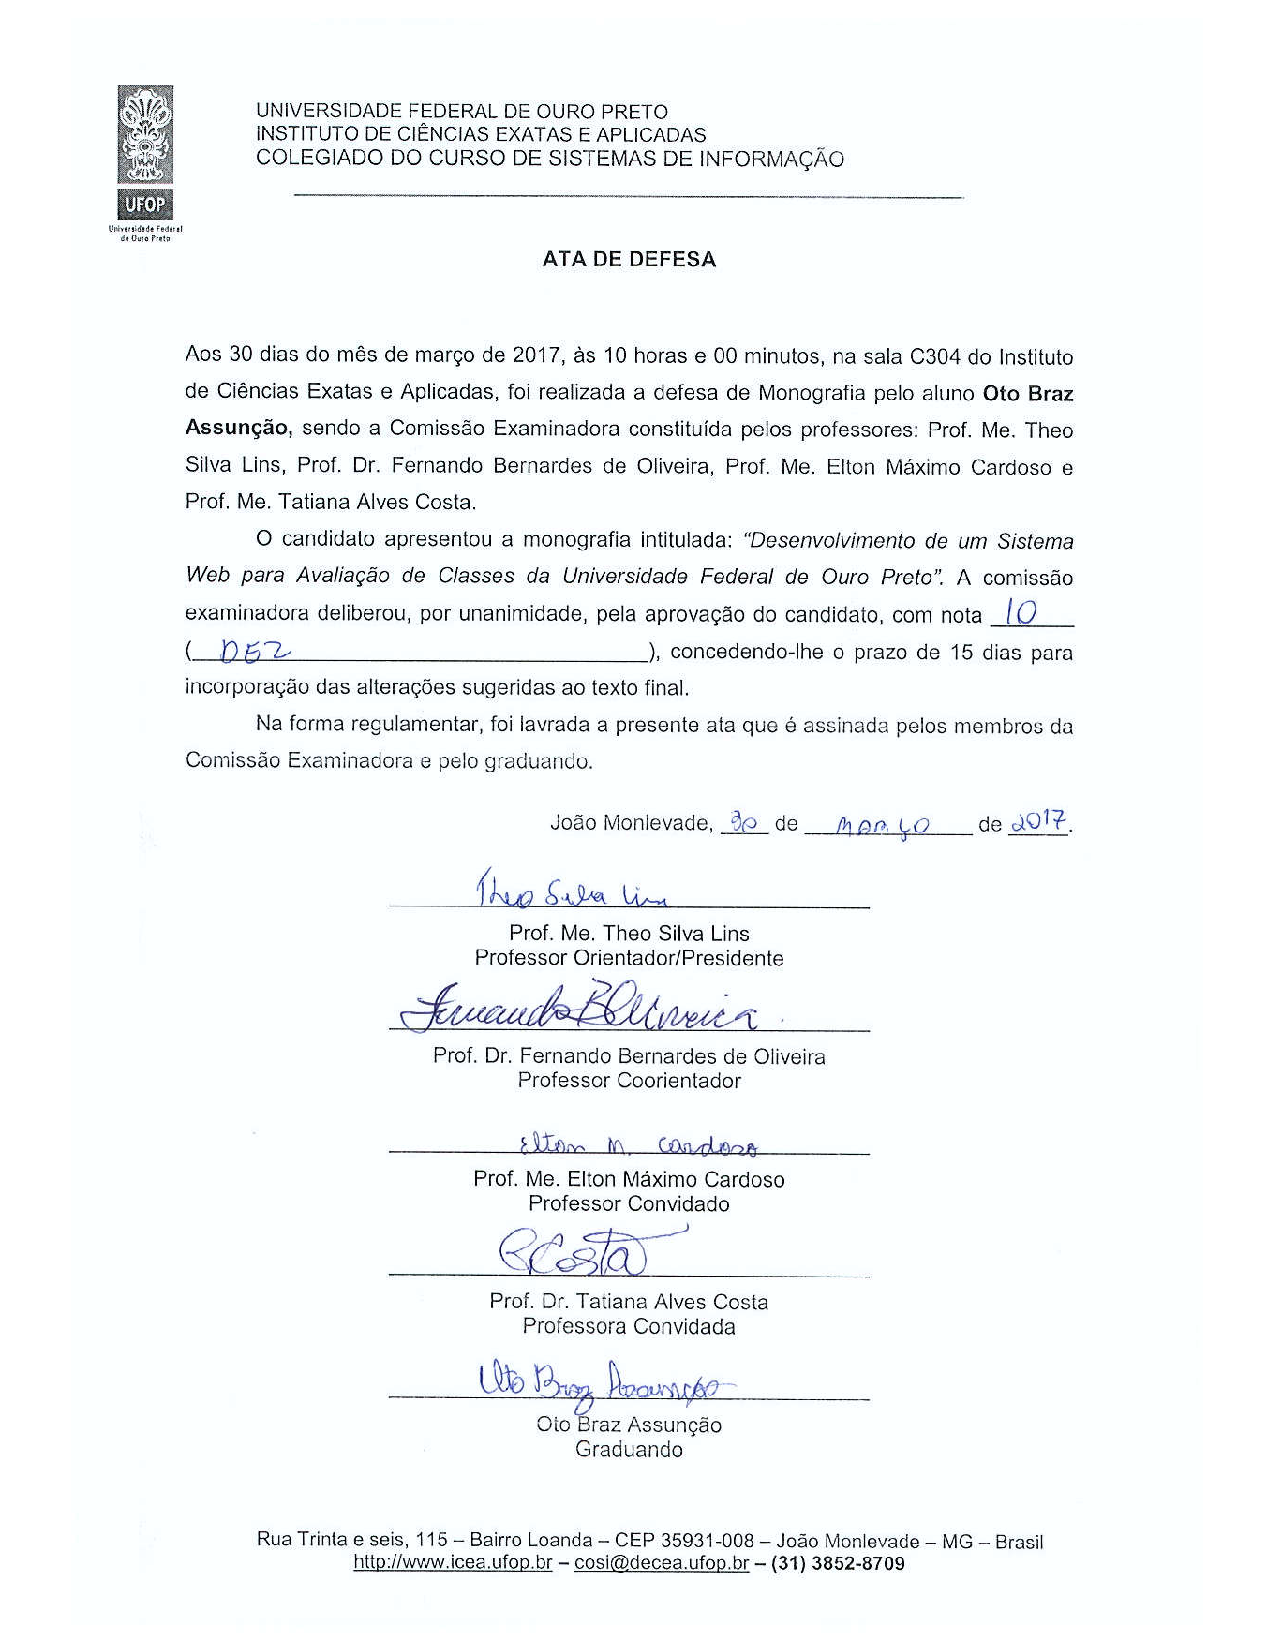
\includepdf{atadefesa.pdf}

% ---
% Agradecimentos
% ---
\begin{agradecimentos}

Aos meus pais Ivete e Karil, minha irmã Luiza e a toda minha família que, com muito carinho e apoio, não mediram esforços para que eu chegasse até esta etapa de minha vida. 

A todos os professores do curso, que foram tão importantes na minha vida acadêmica e no desenvolvimento desta monografia. Em especial ao professor Alexandre Magno, exemplo de superação e dedicação, obrigada pelos concelhos, pelo incentivo e amizade.

A minha maravilhosa e eterna amiga Verônica, 

Ao Bruno Lacerda, que foi parceiro durante toda minha graduação e que agora encerra essa conquista ao meu lado. Você sempre será meu grande amigo!

Aos meus amigos do Laboratório iMobilis, amigos que sempre me ajudaram e com quem pude aprender muitas coisas. Vocês são o melhor time do mundo!

Meus agradecimentos aos amigos da salinha de estudos, companheiros durante grande parte da graduação. Amigos que pude contar, que me ajudaram e aconselharam durante a graduação e quem me espelhei bastante.

À melhor república Mandala, que demonstraram que amizades e companheirismo, mesmo que dotados de muitas diferenças pessoais, são os elementos essenciais para o convívio em grupo, além da irmandade que nos une. Especialmente, agradeço a amiga Pâmela por ter me acolhido e por todos os abraços e insultos carinhosos que trocamos ao longo do curso.

Agradeço ao meu namorado e companheiro Rafael Bortoline, aquele que eu tive a grande sorte de conhecer, alguém responsável por me fazer acreditar que os obstáculos são a nossa força.  

E finalmente, agradeço aos meus orientadores Fernando Bernardes de Oliveira e João Pedro por terem aceitado a minha proposta, acreditarem na minha capacidade para desenvolver este projeto e terem me auxiliado e guiado durante o decorrer no trabalho.

A todos, o meu muito obrigado!


\end{agradecimentos}
% ---

% ---
% Epígrafe
% ---
\begin{epigrafe}
    \vspace*{\fill}
  \begin{flushright}
    \textit{``An expert is one who knows more and more\\
    about less and less until he knows\\
    absolutely everything about nothing.''\\
    (Nicholas Murray Butler)}
  \end{flushright}
\end{epigrafe}
% ---

% ---
% RESUMOS
% ---

% resumo em português
\setlength{\absparsep}{18pt} % ajusta o espaçamento dos parágrafos do resumo
\begin{resumo}

%  Segundo a \citeonline[3.1-3.2]{NBR6028:2003}, o resumo deve ressaltar o
%  objetivo, o método, os resultados e as conclusões do documento. A ordem e a extensão
%  destes itens dependem do tipo de resumo (informativo ou indicativo) e do
%  tratamento que cada item recebe no documento original. O resumo deve ser
%  precedido da referência do documento, com exceção do resumo inserido no
%  próprio documento. (\ldots) As palavras-chave devem figurar logo abaixo do
%  resumo, antecedidas da expressão Palavras-chave:, separadas entre si por
%  ponto e finalizadas também por ponto.

%resumo ttc1
Este artigo apresenta o desenvolvimento de uma plataforma para o gerenciamento de faltas dos alunos pelos professores do Instituto de Ciências Exatas e Aplicadas (ICEA). A plataforma tem como finalidade facilitar o processo de lançamento e acompanhamento das faltas, usando o mesmo sistema de autenticação do portal Minha UFOP como acesso, tornando a experiência do usuário mais agradável. Os professores poderão controlar de maneira mais práticas as faltas, além dos alunos também acompanharem os lançamentos diariamente. Ao invés do lançamento de faltas ocorrer ao final do semestre, os professores farão a chamada por meio do site em sala de aula, que atualizará os dados no sistema. Este documento apresenta a primeira parte do trabalho, compondo o levantamento de requisitos, além de apresentar os modelos observados até o momento.

O gerenciamento de faltas de docentes é uma metodologia obsoleta de controlar presenças, é uma das metodologias mais utilizadas para identificação de precariedades e para o aprimoramento do ensino. Na Universidade Federal de Ouro Preto, o Núcleo de Apoio Pedagógico utiliza \textit{Pesquisa de Desenvolvimento das Disciplinas de Graduação da UFOP} como ferramenta para avaliação. Entretanto, a mesma é muito antiga e demonstra não atender as necessidades dos docentes e discentes. Com o propósito de cobrir as limitações da pesquisa atual e beneficiar o ensino da UFOP, foi desenvolvida uma plataforma \textit{web} denominada \textit{SisAV}. A plataforma permite não apenas o gerenciamento de questionários pelo Núcleo de Apoio Pedagógico, mas também que os docentes criem e gerenciem seus próprios questionários do modo que desejarem. Por fim, após desenvolvido o sistema, foi realizada uma reunião com o Núcleo de Apoio Pedagógico de Ouro Preto e a proposta foi apoiada por eles. Ficou previsto o lançamento de um projeto-piloto no Instituto de Ciências Exatas e Aplicadas, o qual consistirá da fase de implantação e utilização do sistema, no primeiro semestre de 2017.

\textbf{Palavras-chaves}: avaliação de classes. questionários. sistema web. desenvolvimento web.
\end{resumo}

% resumo em inglês
\begin{resumo}[Abstract]
 \begin{otherlanguage*}{english}
   
   The assessment of classes and professors are one of the most used techniques to the identification of issues and improvement of the teaching. The Federal University of Ouro Preto's Pedagogy Support Center has been using the \textit{Pesquisa de Desenvolvimento das Disciplinas de Graduação da UFOP} as the university's classes assessment tool. Nevertheless, this survey is far outdated and has not been meeting the necessities of professors and students. Therefore, in order to fulfill the requirements, which are not being met, and to benefit the teaching in the Federal University of Ouro Preto, it was developed a web system called \textit{SisAV}. The website allows not only the survey management by the Pedagogy Support Center, but also the professors to create and manage their own surveys however they want to do. Finally, after developing the application, a meeting with the Pedagogy Support Center was held and they supported the idea. It is expected that a pilot project, which will consist of deploying and using the system, is going to be conducted on the first semester of 2017 in the Institute of Exact and Applied Sciences.
   
   \vspace{\onelineskip}
   \noindent
   \textbf{Key-words}: classes assessment. surveys. web system. web development.
 \end{otherlanguage*}
\end{resumo}

% ---
% inserir lista de ilustrações
% ---
\pdfbookmark[0]{\listfigurename}{lof}
\listoffigures*
\cleardoublepage
% ---

% ---
% inserir lista de tabelas
% ---
\pdfbookmark[0]{\listtablename}{lot}
\listoftables*
\cleardoublepage
% ---

% ---
% inserir lista de abreviaturas e siglas
% ---
\begin{siglas}
  \item[CRUD] \textit{Create, Read, Update and Delete}
  \item[CSV] \textit{Comma-Separated Values}
  \item[DAP] \textit{Directory Access Protocol}
  \item[DIT] \textit{Directory Information Tree}
  \item[DNS] \textit{Domain Name System}
  \item[EER] \textit{Enhanced Entity-Relationship}
  \item[GUI] \textit{Graphical User Interface}
  \item[HTML] \textit{HyperText Markup Language}
  \item[HTTP] \textit{Hypertext Transfer Protocol}
  \item[ICEA] Instituto de Ciências Exatas e Aplicadas
  \item[IP] \textit{Internet Protocol}
  \item[LDAP] \textit{Lightweight Directory Access Protocol}
  \item[ADMINLTE] \textit{Free bootstrap theme}
  \item[MVC] \textit{Model-View-Controller}
  \item[NAP] Núcleo de Apoio Pedagógico
  \item[NTI] Núcleo de Tecnologia da Informação
  \item[OSI] \textit{Open Systems Interconnection}
  \item[PDF] \textit{Portable Document Format}
  \item[PDDGU] Pesquisa de Desenvolvimento de Disciplinas da Graduação da UFOP
  \item[PHP] \textit{Hypertext Preprocessor}
  \item[PROGRAD] Pró-Reitoria de Graduação
  \item[SGBD] Sistema de Gerenciamento de Banco de Dados
  \item[SI] Sistema de Informação
  \item[SQL] \textit{Structured Query Language}
  \item[TCP] \textit{Transmission Control Protocol}
  \item[TI] Tecnologia da Informação
  \item[UFOP] Universidade Federal de Ouro Preto
\end{siglas}
% ---

% ---
% inserir lista de símbolos
% ---
% \begin{simbolos}
%   \item[$ \Sigma $] Letra grega Sigma
% \end{simbolos}
% ---

% ---
% inserir o sumario
% ---
\pdfbookmark[0]{\contentsname}{toc}
\tableofcontents*
\cleardoublepage
% ---

% ----------------------------------------------------------
% ELEMENTOS TEXTUAIS
% ----------------------------------------------------------
\textual

% ----------------------------------------------------------
% Introdução (exemplo de capítulo sem numeração, mas presente no Sumário)
% ----------------------------------------------------------
\chapter[Introdução]{Introdução}
%tcc1
O objetivo deste trabalho é projetar um sistema de gerenciamento online de faltas para os alunos e os professores do ICEA. O gerenciamento de faltas é um dos maiores problemas enfrentados nas universidades, já que prejudica os alunos que não tem controle sobre elas, acarretando reprovações por falta. O controle manual também resulta transtorno aos professores que ministram aulas em diversas turmas, os quais dependem de suas listas de chamadas impressas ou planilhas para gerenciá-las.

% FBO: este parágrafo está um pouco confuso. :)
% BCA: esta parte foi reescrita
No contexto atual da UFOP, somente ao fim do semestre o total de faltas de cada aluno é lançado pelo professor no sistema MinhaUfop. Desse modo, os alunos não acompanham durante o semestre o número de faltas em um portal, somente consultando cada professor para saber o número de faltas até o momento. Uma vez que a proposta desse sistema seja o controle online, os professores farão a chamada pela plataforma web e os alunos poderão acompanhar suas presenças atualizadas em tempo real. Logo, o objetivo consiste em apresentar a relação de faltas aos alunos para que eles gerenciem e controlem suas faltas.

O restante do artigo é organizado como segue. A Seção \ref{sec:problema} apresenta o problema em estudo e as questões associadas, como o cadastro de faltas para turmas com mais de um professor, como aulas práticas e teóricas, e a atualização dos alunos cadastrados na turma que são matriculados depois e os que trancaram matrícula. Os objetivos gerais e específicos do trabalho são explanados e discutidos na Seção \ref{sec:objetivos}. As etapas desenvolvidas até o presente momento são apresentadas na Seção \ref{sec:etapas}. A Seção \ref{sec:avaliacao} apresenta a avaliação do andamento do trabalho, além das considerações finais desse projeto, bem como as etapas futuras para conclusão do projeto.
%


Docentes em escolas e universidades geralmente possuem o conhecimento de quais são as metodologias de ensino mais benéficas para facilitar o aprendizado deles mesmos. No entanto, segundo \citeonline[p. 8]{fry:2009}, eles tendem a não considerar diretamente qual é a maneira mais eficiente a fim de contribuir para o aprendizado dos discentes de suas classes. Além disso, pouco são feitas análises com o propósito de identificar se a metodologia empregada no momento está sendo efetiva ou não. 

Existem diversos modos de avaliar o ensino, tais como a análise das notas dos discentes, aplicação de questionários e observação dos docentes durante as aulas. A utilização de questionários, especificamente, é bastante comum em diversas instituições de ensinos tanto no Brasil quanto no mundo. Estes se caracterizam pela simplicidade, rapidez de desenvolvimento e capacidade de obtenção de um grande volume de dados relevantes em pouco tempo. Assim, caso estes questionários sejam bem utilizados pelas instituições, eles podem ser responsáveis por oferecer informações importantes aos interessados, sendo os mesmos, em sua grande maioria, os docentes, discentes e pedagogos da instituição.

De acordo com \apudonline{ramsden:1992}{fry:2009}, as avaliações de classes são fundamentais para um ensino de qualidade, contribuindo para o entendimento de como as metodologias dos docentes afetam o aprendizado dos discentes. Um dos fatores que definem a eficiência de uma avaliação é o grau de relevância dos dados obtidos pela mesma. Ademais, caso os dados sejam apresentados de modo amigável, facilitando o processo de análise, as conclusões obtidas podem ser ainda mais precisas. Levando estes pontos em consideração, fazer o uso de sistemas computacionais para o gerenciamento de questionários pode ser extremamente benéfico as instituições de ensino.

A Tecnologia da Informação (TI) é ``todo \textit{software} e \textit{hardware} de que uma empresa necessita para atingir seus objetivos organizacionais'' \cite[p. 12]{laudon:2010}. Presentemente, a TI se tornou essencial às organizações uma vez que ela é capaz de automatizar e facilitar a realização de diversas atividades. Todavia, simplesmente fazer o uso básico da TI pode não atender completamente as necessidades de uma entidade, especialmente aquelas que lidam com um grande fluxo de dados e precisam gerenciar informações de maneira eficiente. Por informação, entende-se todos dados processados e que são relevantes àqueles que os utilizam. Sistemas que gerenciam a informação são chamados de Sistemas de Informação (SI). Segundo \citeonline[p. 12]{laudon:2010} um SI é ``um conjunto de componentes inter-relacionados que coletam (ou recuperam), processam, armazenam e distribuem informações''. Estas informações, por sua vez, são geralmente utilizadas durante o processo de tomada de decisões dentro das organizações.

O presente trabalho aborda o desenvolvimento de um sistema \textit{web} para o gerenciamento de questionários na Universidade Federal de Ouro Preto (UFOP). Com o objetivo de facilitar a integração do sistema à UFOP foi determinado que o acesso ao mesmo fosse realizado por meio das credenciais da plataforma \textit{minhaUFOP} utilizadas pelos docentes, discente e outros funcionários da instituição. 

    \section{Problema}
    %tcc1
    
Com o grande número de alunos que são matriculados em uma turma, a chamada de faltas fica custosa para professores que lecionam para várias turmas, e depois precisam contabilizar os lançamentos. Como solução para atender a esse tipo de demanda surgiu a necessidade de um Sistema Integrado de Gestão (SIG), que fornecerá um portal para registrar a quantidade de faltas ao longo do tempo, podendo assim gerar relatórios e estudos para a analise do número de faltas.

A plataforma tem características importantes que devem ser consideradas, tais como: o registro de faltas para turmas com mais de um professor vinculado e a verificação do limite de faltas dos alunos. Portanto, o modelo de dados considera que uma disciplina pode ter mais de um professor. Por exemplo, uma turma pode ter dois professores, sendo um para aula prática e outra para teórica. E a segunda característica está na tabela de disciplinas, que possui o número limite de faltas para aprovação, que quando é atingido, tanto o aluno quanto o professor serão notificados, esse recurso é essencial para identificar alunos que desistiram da disciplina ou trancaram matrícula. Tais peculiaridades são fundamentais para o gerenciamento e garantia da completude do escopo do trabalho. %BCA: acredito que desvincular o aluno(deixar de lançar a falta) que atingiu o limite é muito rigoroso, já que esse aluno pode vir a abonar faltas futuramente. Mas depois de notificá-los, o que pode ser feito????

    

    A UFOP faz o uso de uma avaliação e acompanhamento semestral das disciplinas chamada \textit{Pesquisa de Desenvolvimento de Disciplinas da Graduação da UFOP} (PDDGU). A pesquisa possui duas versões, ambas possuindo dez questões fechadas. Uma delas é referente a avaliação que os docentes fazem das turmas que eles lecionaram em determinado semestre, enquanto que a outra é direcionada a avaliação que os discentes fazem dos docentes responsáveis por ministrar as aulas de suas turmas.

    Durante este trabalho, foi aplicado um questionário aos docentes do Instituto de Ciências Exatas e Aplicadas (ICEA) a fim de saber a opinião dos mesmos a respeito da PDDGU que é respondida pelos discentes. As respostas deram indícios que a pesquisa é limitada e ineficiente. Ela não possui questões subjetivas e deixa de abordar diversos tópicos que seriam mais relevantes aos docentes interessados. Logo, os discentes não podem expressar bem suas opiniões, dificultando, para docentes e o Núcleo de Apoio Pedagógico (NAP), a identificação de pontos a serem melhorados. Ainda, uma das grandes queixas é que ela apenas pode ser respondida ao fim do semestre. Todos docentes que responderam o questionário aplicado consideram que as notas dos alunos possuem grande influência nas respostas, levando a um viés dos resultados obtidos pela pesquisa da UFOP. 

    A apresentação dos resultados também não é ideal. No presente momento, faz-se o uso de uma simples tabela com a porcentagem das respostas de cada opção das perguntas do questionário. A estruturação dos resultados não é boa e dificulta o processo de interpretação e análise dos mesmos. Uma boa apresentação dos resultados obtidos é essencial àqueles que os analisarão.

    \section{Objetivos}

        Nesta seção, são apresentados os objetivos gerais e específicos do trabalho desenvolvido.

        \subsection{Objetivo Geral}

    O objetivo do trabalho é o desenvolvimento de uma plataforma \textit{web} para avaliação de classes da UFOP e o gerenciamento e divulgação de orientações realizadas. A plataforma será utilizada por docentes, discentes e pelo NAP. Os docentes e o NAP poderão elaborar questionários e disponibilizá-los às turmas e os discentes poderão respondê-los. Por fim, os resultados dos questionários serão apresentados por meio de gráficos aos usuários do sistema.
    
    %tcc
    O objetivo deste projeto é a modelagem e a implementação de uma plataforma online prática e funcional para gerenciamento de faltas. A aplicação permitirá o lançamento diário das faltas pelos professores e o monitoramento e controle das faltas pelos alunos. O objetivo neste relatório é apresentar de forma clara e simplificada as diversas etapas que são necessárias para o desenvolvimento em uma plataforma deste tipo, desde a análise até ao desenvolvimento propriamente dito.

        \subsection{Objetivos Específicos}
        
        


            Os objetivos específicos do trabalho são:
      
            \begin{itemize}
            	\item Permitir que o NAP elabore e disponibilize questionários a universidade.
                \item Permitir que os docentes criem seus próprios questionários de avaliação de classes.
                \item Permitir que os discentes respondam aos questionários de suas classes.
                \item Apresentar os resultados dos questionários amigavelmente tanto para todos os usuários do sistema.
                \item Facilitar a detecção de precariedades a partir no ensino a partir dos resultados.
                \item Fornecer meios para que discentes tenham maior conhecimento das orientações realizadas no ICEA.
                \item Facilitar a busca de possíveis orientadores por parte dos discentes.
                
                
                %tcc                      
            
\item Levantamento de requisitos para entender o ambiente de negócios do software. Ela permite que se consiga ter uma percepção ampla sobre os resultados solicitados e sobre as principais funcionalidades esperadas.

\item Implementar todas as funcionalidades propostas para ambos os módulos, um dedicado aos discentes e outro aos docentes da instituição, garantindo que a plataforma seja integrada.

\item Escrever cenários de testes e executá-los, a partir da ferramenta Selenium-IDE, utilizada para testes funcionais automatizados através do navegador. Avaliando o desempenho e identificando possíveis falhas da aplicação proposta. 

\item Analisar e discutir os resultados obtidos, além de identificar possíveis melhorias e considerações gerais sobre o processo.
            \end{itemize}


    \section{Justificativa}

        Com a finalidade de atender a necessidade da melhoria contínua do ensino na UFOP, a utilização do sistema desenvolvido, juntamente com a PDDGU, se faz importante para a instituição. Levando em consideração que a plataforma utilizará metodologias diferentes, permitindo a adaptação de questionários e utilização de questões abertas e fechadas, além de fornecer \textit{feedback} relevante aos interessados, é esperado que a implantação da mesma contribua positivamente para as atividades realizadas na UFOP, sendo elas classes ou orientações.

    \section{Estrutura do Trabalho}

        O trabalho é estruturado em quatro capítulos, sendo o primeiro deles responsável por introduzir o projeto desenvolvido. No Capítulo \ref{ref_teoricos} é discorrido a repeito da fundamentação teórica do trabalho. Em seguida, o Capítulo \ref{metodologia}, detalha toda a metodologia utilizada para o desenvolvimento do projeto. Por fim, são apresentadas as considerações finais no Capítulo \ref{conclusao}.

% ---
\chapter{Referenciais teóricos}\label{ref_teoricos}
% ---

	Este capítulo apresenta toda a fundamentação teórica do projeto. São discutidas as metodologias de gerenciamento de faltas pelos docentes nas instituições de ensino, ferramentas e tecnologias utilizadas para o desenvolvimento e sistemas correlatos.

    \section{Controle de Frequência}

        O gerenciamento de faltas é fundamental para auxiliar docentes e discentes, já que o número de faltas é considerado como critério de avaliação para a aprovação nas disciplinas. Usar um sistema para controle de frequência escolar também é prático para a instituição de ensino, pois com o histórico de frequência dos alunos, a universidade pode gerar arquivos para utilização por professores e gestores, além de facilitar a visualização de estatísticas, dados e metas e acompanhamento dos discentes.
               
        Existem inúmeras maneiras de gerenciar as faltas, seja por planilhas, documentos online e até mesmo o método mais antigo, o papel. As instituições de ensino em geral têm em seu portal o diário de frequência, o que facilita o controle dos alunos. Definir qual metodologia deverá ser usada dependerá de diversos fatores: a cultura institucional, a qualidade do processo, a usabilidade do sistema, etc. 
                
        Dessa forma, o processo atual de gerenciar faltas pode ser feito por planilhas ou no papel, sendo assim, o professor tem acesso a relação de alunos matriculados e conforme escolha dele, o docente poderá gerenciar as faltas pela própria planilha, ou a partir da impressão da mesma, de modo que o professor registre as faltas e as contabilize, para que ao final do semestre letivo, seja entregue o relatório impresso ao colegiado, ao qual é responsável por aprovar o documento. 
        O Diário de Frequência é uma plataforma \textit{web} desenvolvida especificamente para a UFOP do campus ICEA e diante dessa característica o sistema foi criado atendendo o processo atual de chamada. Ou seja, o documento impresso usado hoje com a relação de faltas será substituído pelo relatório gerado pelo sistema. 
        
        Contudo, o NTI foi contactado para que a proposta desse projeto fosse validada, permitindo assim, que a proposta fosse executada, já que atualmente nada tem sido desenvolvido para controlar faltas nos cursos presenciais.
        
        \subsection{Levantamento de Requisitos junto aos professores do ICEA }
        
        O diário de frequência do ICEA é um sistema para registrar e controlar as faltas dos alunos. Este sistema importa para sua base de dados as planilhas das turmas em que os docentes lecionam e a partir da lista de alunos matriculados é realizada a chamada online. Os discentes podem acompanhar o número de faltas para cada disciplina em que ele esta matriculado, desde que os seus professores utilizem o sistema.

		Diante dessa problemática foi discutido e levantado requisitos essenciais para a aplicação e quais funcionalidades o sistema contemplaria. 
        
        Os principais requisitos levantados são:
      
            \begin{itemize}
            	\item Importar planilha da turma para fazer chamada 
                \item Registrar falta diária ou por intervalo de dias
                \item Anexar atestado para solicitar abono de faltas
                \item Acompanhamento do número de faltas 
            \end{itemize}
                
        

    \section{UFOP Boilerplate}
    
    Para simplificar o processo de autenticação dos sistemas web desenvolvidos para a comunidade acadêmica da UFOP, foi criado um boilerplate(https://github.com/jpmoura/ufop-boilerplate-laravel), um template front-end para a criação de sites da Web, rápidos, robustos e adaptáveis.
    
    Esse boilerplate contém somente a parte lógica da autenticação modelada para o Laravel 5.3, geração otimizada dos assets e alguns tratamentos de eventos usando log, que são exemplos bem simples de uso do framework.

	Ele usa a mesma autenticação do Minha UFOP, ou seja, é extensível a toda universidade e não somente ao campus ICEA. Essa autenticação é feita através da API LD(AP)I(https://github.com/jpmoura/ldapi ), desenvolvida por Plinio e Joao Pedro.    

        \subsection{Frameworks e Desenvolvimento Web}
        
            A utilização de \textit{frameworks} no desenvolvimento \textit{web} é imensa e se faz essencial para o sucesso da aplicação. Já que ele destina-se a aliviar a sobrecarga associada a atividades comuns realizadas no desenvolvimento. 
            
            A maioria dos \textit{frameworks} para desenvolvimento \textit{PHP} se baseiam no padrão de projeto \textit{Model-View-Controller} (MVC). MVC é uma forma de programação que isola a lógica de negócio da camada de exibição. Essa organização faz com que o trabalho seja desenvolvidoe mais rápido e de forma setorizada. 
            
            O MVC foi proposto em 1980 como uma abordagem para design de GUI\footnote{Graphical User Interface}, permitindo múltiplas representações de um objeto e diferentes interações com estas representações'' \cite[p. 432, tradução nossa]{sommervile:2011}. Considerando o domínio dos \textit{websites}, cada componente lógico do MVC pode ser definidos da seguinte maneira:

            \begin{itemize}
              \item \textbf{\textit{Model:}} responsável pelo modelo de dados, gerenciar os dados do sistema.
              \item \textbf{\textit{View:}} responsável pela camada de exibição, definir como os dados serão representados e exibidos ao usuários. É a partir da \textit{view} que o usuários fazem a interação com o sistema.
              \item \textbf{\textit{Controller:}} respinsável pela lógica de negócio, responde às interações do usuário, definindo quais operações serão realizadas, quais dados serão manipulados e quais \textit{views} serão utilizadas para representá-los.
            \end{itemize}

            \citeonline{sommervile:2011} também afirma que, apesar das diferenças, todos os \textit{frameworks} para aplicações \textit{web} geralmente oferecem as seguintes funcionalidades:

            \begin{itemize}
                \item \textbf{\textit{Segurança:}} inclusão de classes para auxiliar o processo de autenticação de usuários e gerenciamento de permissões.
                \item \textbf{\textit{Páginas web dinâmicas:}} capacidade de criação de \textit{templates}, onde somente determinadas partes dos mesmos são alteradas.
                \item \textbf{\textit{Suporte a Banco de Dados:}} Permitem a interação da aplicação com um banco de dados externo, facilitando a execução de consultas e \textit{CRUD} (\textit{Create}, \textit{Read}, \textit{Update}, \textit{Delete}) de registros.
                \item \textbf{\textit{Gerenciamento de sessões:}} possuem classes para definir e gerenciar sessões dos usuários.
                \item \textbf{\textit{Interações de Usuário:}} suporte à AJAX para criação de páginas mais interativas.
            \end{itemize}

        \subsection{Laravel} 
		 \textit{Laravel}\footnote{https://laravel.com/} é um \textit{framework}  \textit{open-source}, voltado para \textit{web} e feito em PHP. Foi criado por Taylor Otwell e teve sua primeira versão dispobilizada em 2011,  tendo seu código-fonte hospedado no GitHub. 
         
         Algumas características nativas do \textit{Laravel} são sua sintaxe simples e concisa, o que fez com que nos últimos anos o \textit{framework} evoluisse rapidamente, se tornando bastante popular entre os desenvolvedores \textit{PHP}, como aponta a pesquisa recente do Sitepoint\footnote{https://www.sitepoint.com/best-php-framework-2015-sitepoint-survey-results/} que mostrou que é o framework mais popular de 2015.
         
         Assim como grande maioria dos \textit{frameworks} para aplicações \textit{web}, o \textit{Laravel} também segue o padrão MVC e tem uma série de características que tornam possível o desenvolvimento rápido de aplicações. Uma das grandes vantagens desse \textit{framework} é a criação de \textit{migrations}, que basicamente são um controle de versão para o banco de dados da aplicação. Deste modo, fazer modificações na estrutura do banco de dados e compartilhamento do mesmo entre desenvolvedores se torna algo extremamente simples de ser feito. 
         
         Além disso, para o layout, foi usado como base o design \textit{AdminLTE}\footnote{https://adminlte.io/themes/AdminLTE/documentation/index.html} desenvolvido por Abdullah Almsaeed\footnote{mailto:abdullah@almsaeedstudio.com}, utilizando uma versão personalizada da dashboard do AdminLTE 2, template que já está sendo usado nas aplicações desenvolvidas para o campus ICEA, dessa forma, o gerenciador de faltas seguirá a mesma ideia e padrão de design. 

    \section{Serviços de Diretório e LDAP}

        Um diretório é um banco de dados especializado, construído especificamente para realização de consultas, além de fornecer operações básicas de atualização'' \cite[p. 3, tradução nossa]{openLdap:2011}.

        De acordo com \citeonline{openLdap:2011}, o \textit{Lightweight Directory Access Protocol} (LDAP) é um protocolo leve utilizado para fazer acesso a serviços de diretório to tipo \textit{X.500}, geralmente utilizando conexões orientadas a transferência de serviços tais como \textit{TCP/IP} e do modelo cliente-servidor. Os serviços de diretório \textit{X.500}, também chamados de serviços de diretório OSI, possuem um Protocolo de Acesso à Diretórios (DAP) entre o \textit{gateway} e servidor. Entretanto, este DAP é pesado e consume muitos recursos. A vantagem que o LDAP possui é a pequena utilização de recursos ao mesmo tempo que fornece a maioria das funcionalidades do DAP. 

        As informações no LDAP são baseadas em entradas, as quais possuem, além dos atributos comuns, um atributo especial chamado \textit{Distinguished Name} (DN). O DN é usado para referenciar uma entrada. Cada entrada no LDAP é organizada através de árvores hierárquicas chamadas \textit{Directory Information Trees} (DIT). Segundo a \citeonline{openLdap:2011}, a abordagem de utilizar os nomes dos domínios da Internet para construção de DITs tem se tornado comum já que elas permitem o uso do Domain Name System (DNS) para localizar os serviços de diretório. A Figura \ref{fig:ldap_tree} mostra uma DIT que faz uso da nomenclatura da Internet:

        \begin{figure}[h]
           \centering
           \caption{Árvore de Diretórios LDAP (nomenclatura da Internet)}\label{fig:ldap_tree}
           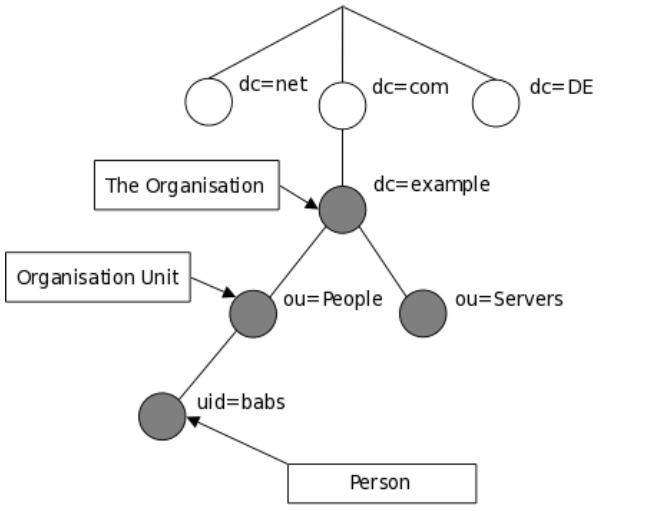
\includegraphics[scale=0.6]{img/ldap_tree}
           \subcaption*{Fonte: \citeonline[p. 5]{openLdap:2011}}
        \end{figure}
        
        
Com base nisso, para a sessão de autenticação usando os dados do Minha UFOP, foi usada a \cite{API-LDAP} como API de autenticação, que atualmente está hospedada nos servidores do campus do ICEA. Permitindo que com os mesmos dados de acesso ao portal já existente, o diário também seja acessado.

        \subsection{OpenLDAP na UFOP}

        OpenLDAP\footnote{openldap.org} é uma implementação \textit{open-source} do LDAP. A UFOP utiliza o \textit{OpenLDAP 2.4} para armazenar diversas informações sobre a universidade. A DIT utilizada pela UFOP possui informações sobre três tipos de : \textit{grupos}, \textit{maquinas} e \textit{people}. Todavia, apenas as unidades \textit{grupos} e \textit{people} foram utilizadas neste trabalho.

        A unidade organizacional \textit{grupos} faz referência aos grupos em que as diversas pessoas relacionadas a UFOP pertencem: cursos oferecidos, departamentos, áreas de atuação de técnicos, equipe pedagógica, etc. 

        A unidade \textit{people} possui informações relativas a todos aquelas dentro da UFOP, docentes, discentes, técnicos, etc. As principais informações armazenadas nesta unidade são: \textit{cpf, nome, grupo pertencente, campus e e-mail}. Além disso, informações utilizadas para realização da autenticação em sistemas da faculdade tais como a \textit{minhaUFOP} também estão armazenadas nesta unidade.

    \section{Banco de Dados}
   
   Um banco de dados é uma estrutura, física ou lógica, responsável pelo armazenamento de registros com a finalidade dos mesmos serem consultados quando necessário. Um dos principais recursos utilizados por SIs é o banco de dados digital. Estes possuem inúmeros dados referentes a um tipo de informação tais como clientes, fornecedores, produtos, etc. Cada um destes tipos é comumente chamado de \textit{entidade}, enquanto que, cada característica que determinada entidade possui é denominada \textit{atributo} \cite[p. 145]{laudon:2010}.
   
	Dentre os diversos tipos de banco de dados, os bancos de dados relacionais são os mais utilizados mundialmente. Eles ``organizam os dados em tabelas bidimensionais (denominadas relações) com colunas e linhas. Cada tabela contém dados referentes a uma entidade e seus atributos'' \cite[p. 145]{laudon:2010}. 

	Com o objetivo de gerenciar os bancos de dados computacionais, Sistemas de Gestão de Banco de Dados (SGBD) foram criados. Os SGBDs permitem que os usuários executem tarefas tais como armazenamento, organização, adição, acesso e processamento dos dados de maneira mais simples e eficiente. Durante o trabalho, foram utilizados os SGBDs \textit{MySql}, que estava instalado no servidor para testes, e \textit{MariaDB}, que estava instalado no ambiente de desenvolvimento.  
   
   \subsection{MySQL}
      
      O \textit{MySQL}, segundo \citeonline{mysql:2017}, é desenvolvido, distribuído e mantido pela Oracle Corporation\footnote{www.oracle.com}, sendo o SGBD com a versão \textit{open-source} mais popular do mundo, fazendo uso da Structered Query Language (SQL), que é a linguagem de manipulação de dados utilizada pela maioria dos SGBDs.
      
      \subsection{MySQL WorkBench}
      importação das migrations, plugin Laravel
      MariaDB Server\footnote{mariadb.org} é um servidor de banco de dados completamente \textit{open-source} criado pelos mesmos desenvolvedores do \textit{MySQL}. Conforme \citeonline{aboutmariadb:2016}, ele é capaz de substituir completamente o \textit{MySQL} e o processo de atualização e substituição do sistema do banco de dados é trivial. O \textit{MariaDB}, de acordo com \citeonline{featuresmariadb:2016}, é basicamente um \textit{MySQL} melhorado, sendo mais rápido e possuindo diversos mecanismos de armazenamento e funcionalidades além daquelas suportadas pelo \textit{MySQL}.
      
    \section{Servidores Web}

        Servidores \textit{web} permitem que as pessoas acessem os \textit{websites} na internet. Eles processam as requisições dos usuários via \textit{Hypertext Transfer Protocol} (HTTP), que é o protocolo utilizado para transferência de informações pela internet. A expressão \textit{Servidor Web} pode referenciar duas tecnologias: \textit{computador (hardware)} ou \textit{programa (software)}. 

        O servidor \textit{web} (computador) possui diversos \textit{websites} hospedados e permanece conectado a todo instante, permitindo que os usuários consigam acessar os \textit{websites} nele armazenados sempre que necessitarem.  

        O servidor \textit{web} (programa) é o \textit{software} que fica em execução no computador responsável por hospedar os \textit{websites}. A principal função dele é servir as páginas \textit{web}, ou seja, ele fica sempre no aguardo de requisições feitas pelos usuários (clientes) e responde a essas requisições.

        \subsection{Apache HTTP Server}

        Segundo a \citeonline{aboutapache:2016}, o \textit{Apache HTTP Server Project}\footnote{httpd.apache.org} é um projeto que conta com a colaboração de desenvolvedores de  várias partes do mundo, buscando o desenvolvimento e manutenção constante de um servidor HTTP \textit{open-source} para atender sistemas operacionais modernos. O objetivo do projeto é a disponibilização de um servidor HTTP seguro, eficiente e extensível, sempre estando a par com os padrões atuais HTTP. 

       O servidor desenvolvido veio a ser chamado \textit{Apache HTTP Server} (httpd). Ele foi lançado em 1995 e ganhou popularidade em um curto espaço de tempo, se tornando o servidor \textit{web} mais popular na Internet \cite{aboutapache:2016}. Atualmente, o mesmo se encontra na versão 2.4, a mesma utilizada durante o desenvolvimento deste trabalho. 

    \section{Sistemas Correlatos}

       Nesta seção serão apresentados alguns sistemas correlatos à plataforma desenvolvida. A correlação existem devido a um dos seguintes fatores: funcionalidades, métodos empregados e aplicação.     
       

%Como trabalhos relacionados, foram encontradas três aplicações de serviços de faltas, tanto no mercado quanto na própria instituição, e somente uma sendo para o lançamento de faltas pelo professor. Uma breve descrição das aplicações é abordada abaixo.

        \subsection{Formei UFOP}
        O \textit{FormeiUFOP} é o nome da aplicação móvel desenvolvida por \citeonline{enio:2016} como trabalho de conclusão do curso de Sistemas de Informação da UFOP. O sistema tem como objetivo facilitar o gerenciamento de notas do campus ICEA. 
        
        O aplicativo móvel é voltado para os estudantes da UFOP acompanharem seu progresso acadêmico, desenvolvido com o principal objetivo de planejar e gerenciar o progresso dos discentes. Podendo o discente avaliar seu desempenho escolar, definir suas prioridades de disciplinas a cada semestre e prever o término do curso. Esse trabalho, tem como um de seus objetivos futuros, a criação do controle de faltas, sendo atingido na proposta desse trabalho.
               
        A motivação do \textit{FormeiUFOP} está no fato em que nas universidades os discentes são responsáveis por escolherem grande parte das disciplinas que eles cursarão ao longo de sua vida acadêmica. Logo, a plataforma veio para facilitar e auxiliar os estudantes a decidir quais disciplinas eles faram para adiantar o curso. Tem-se como trabalhos futuros, o controle de faltas online do ICEA, sendo contemplado nesse projeto.

        \subsection{Presente!}
         O \textit{Presente!}\footnote{http://www.ufla.br/ascom/2016/04/26/volta-as-aulas-estudante-da-ufla-cria-aplicativo-para-auxiliar-no-controle-de-faltas/} é uma ferramenta gratuita que auxilia os discentes no controle das faltas em cada disciplina matriculada. Com o aplicativo, os próprios usuários cadastram as matérias que estão cursando naquele período e os respectivos dias das aulas; então, eles receberão notificações no celular perguntando se houve frequência na referida aula cadastrada. O aplicativo é gratuito e \textit{open-source}.

        Apesar de todos os pontos positivos mencionados, utilizar o \textit{Presente!} para gerenciar faltas não é eficiente visto que ele depende do aluno para registrar suas faltas e esse controle pode contradizer com o controle dos docentes, existe a possibilidade do aluno esquecer de registrar uma aula que perdeu e acabar faltando em uma aula que seria a última oportunidade para ser aprovado, e ocorrerá a reprovação por falta, já que o limite foi estourado. 
        
        Logo, disponibilizar e gerenciar por parte do docente é mais seguro e o discente fica por conta de analisar os número de faltas e avaliar se poderá faltar ou não, bem como gerenciá-las, o que é uma tarefa fácil.

        \subsection{Minha UFMG}
        
		O \textit{MinhaUFMG} é um portal online para atender a todos os professores, funcionários e alunos da instituição, fornecendo um conjunto de ferramentas de trabalho colaborativo, como: correio eletrônico, agenda corporativa, controle de tarefas, notas e faltas pelo professor. O \textit{MoodleUFOP} que também fornece as funcionalidades do MinhaUFMG, não conta com o controle de frequência para os cursos presenciais, deixando que o controle de faltas a critério do professor, sendo através do diário impresso ou planilhas.
        
        Similarmente a\footnote{https://github.com/chesman12/ufop-faltas}, a aplicação desenvolvida neste trabalho, o \textit{Diário de Frequência} é uma plataforma \textit{web} desenvolvida especificamente para a UFOP e que tem como objetivo automatizar o processo de chamada. 

% ---
\chapter{Metodologia}\label{metodologia}
% ---
        Neste capítulo são detalhadas todas as etapas realizadas durante o desenvolvimento do trabalho. São apresentadas as atividades referentes a revisão teórica, levantamento de requisitos, arquitetura do banco de dados, desenvolvimento do sistema e testes realizados. Por fim, é discutido a respeito da validação do sistema pelos professores.
        
    \section{Implantação da metodologia de desenvolvimento \textit{BOPE}}
    
     O BOPE é um processo híbrido das metodologias ágeis Scrum e XP aliados com as orientações contidas no Project Management Body of Knowledge (PMBOK), um conjunto de diretrizes na gestão de projetos. %citar PMBOK
     
	O fluxo de trabalho do BOPE\cite{PEREIRA; Senna Carneiro; PEREIRA, 2013} determina que  uma série de regras que incluem tarefas de planejamento, execução e testes sejam definidas. Além disso, o mesmo é um processo dirigido por artefatos o que significa que as tarefas realizadas devem gerar um artefato padronizado. Desta forma, foram desenvolvidos cenários e casos de testes (Anexo A), requisitos funcionais e não funcionais (Apêndice A), facilitando a definição das tarefas e atividades a serem concluídas durante o desenvolvimento
deste projeto.

	O desenvolvimento ágil é uma técnica muito eficiente no desenvolvimento de
qualquer tipo de projeto. A possibilidade de gerar artefatos que podem rapidamente se
moldar as necessidades do projeto, permite evitar um cenário onde o produto final nada se
encaixa com o que se era esperado. Uma vez que as etapas de desenvolvimento são curtas,
um erro de planejamento pode ser rapidamente corrigido. Com isso evita-se retrabalho e
consequentemente economiza-se recursos, fazendo com que a chance de sucesso do produto
final seja muito maior.

    \section{Estudo do Escopo e Problema}

    A primeira etapa envolveu pesquisas e revisões da literatura que abordam o problema, escopo do projeto e ferramentas que estão de alguma maneira relacionadas ao trabalho. 

    ''O software tem o único propósito de fornecer valor aos seus usuários'' \cite[tradução nossa]{hooker:1996}. Assim, um dos pilares do projeto são as pessoas que utilizarão o sistema.  e entender o papel de cada uma é fundamental. Levando isso em consideração, foram feitos levantamentos a fim de compreender melhor os pontos de vista dos principais usuários finais do sistema, discentes e docentes.

    O ambiente onde o sistema será implantado é um importante fator e foi considerado. Uma vez que o sistema tem como objetivo atender as necessidades de uma universidade, foram realizados estudos a fim de compreender melhor como é feito o processo de controlar faltas e gerenciar os resultados finais.
    
    \section{Estudo de Ferramentas e Tecnologias}

    Nesta fase foram realizadas pesquisas relativas as ferramentas e tecnologias utilizadas no desenvolvimento do sistema. O principal objetivo deste estudo foi para obtenção de um maior entendimento sobre as vantagens, desvantagens e limitações de cada ferramenta a fim de reduzir a ocorrência de problemas e facilitar a correção dos mesmos quando eles ocorressem.

    As principais tecnologias de desenvolvimento do sistema são as mesmas que estão sendo utilizadas recentemente pelo NTI do ICEA, de modo que fazer a integração, manutenção e expansão do mesmo seja mais simples. As ferramentas e tecnologias utilizadas no ambiente de desenvolvimento do \textit{Sistema de Avaliação} foram:

    \begin{itemize}
        \item \textbf{Plataforma:} \textit{Web};
        \item \textbf{Servidor:} \textit{Apache 2.4};
        \item \textbf{Linguagens:} \textit{PHP 5.6}, \textit{HTML5}, \textit{Javascript}, \textit{Jquery}, CSS;
        \item \textbf{Framework:} \textit{Laravel 5.2} / \textit{Laravel 5.3};
        \item \textbf{Banco de Dados:} \textit{MariaDB 10.1.9},\textit{ MySQL 5.7.17};
        \item \textbf{Serviço de Diretório:} \textit{OpenLDAP 2.3};
    \end{itemize}

    \section{Levantamento de Requisitos}

    ''Os requisitos de um sistema são descrições de funcionalidades e restrições das mesmas, refletindo as necessidades daqueles que o utilizarão'' \cite[p. 83, tradução nossa]{sommervile:2011}. Para facilitar a identificação e definição de requisitos foram realizadas as seguintes atividades: identificação dos \textit{stakeholders}, aplicação de questionários e desenvolvimento de casos de uso das principais funcionalidades do sistema.

    \subsection{Identificação dos \textit{Stakeholders}}

    \citeonline{sommervile:2011} diz que os \textit{stakeholders} são aqueles que são beneficiados pelo sistema tanto direta quanto indiretamente. Os principais \textit{stakeholders} do \textit{Sistema de Avaliação} são: \textit{discentes, docentes, membros do colegiado, responsáveis pelo desenvolvimento do sistema, responsáveis pela manutenção do sistema}.   
    
    
	\subsection{Avaliação da Qualidade do Sistema Web}
     Metodologias e Ferramentas para 
     AVALIAÇÃO DE USABILIDADE.

    \subsection{Usuários do Sistema}

    Após os \textit{stakeholders} serem identificados, foi determinado quais seriam os diferentes tipos de usuário que o sistema possuiria. Os tipos definidos foram: \textit{Administrador}, \textit{Professor} e \textit{Aluno}.

    \begin{itemize}
   		\item \textbf{Administrador: gerenciam novas disciplinas e períodos.} 
        \item \textbf{Professor: } gerenciam turmas e realizam cadastro de faltas. Além disso, eles também aprovam solicitações de abono feitas pelos alunos.
        \item \textbf{Alunos: } acompanham o lançamento de faltas e as gerenciam; solicitam abono de faltas ao professor, desde que tenham atestado ou justificativa válida.
    \end{itemize}   
    

    \subsection{Identificação de Limitações da Aplicação}

    Os principais problemas e limitações da Pesquisa de Desenvolvimento de Disciplinas de Graduação da UFOP foram identificados através do questionário \textit{Pesquisa de Desenvolvimento de Disciplinas da Graduação da UFOP (respondida pelos discentes)} (Apêndice \ref{questionario_1}). Este questionário foi aplicado aos docentes do ICEA a fim de saber a opinião dos mesmos sobre a \textit{Pesquisa de Desenvolvimento de Disciplinas da Graduação da UFOP} que os alunos respondem após cada semestre. 

    A partir das respostas do questionário aplicado, conversas com os docentes e reuniões com os presidentes do colegiado de \textit{Sistemas de Informação} e \textit{Engenharia da Computação}, foram identificados os principais problemas:

    \begin{enumerate}
    \item Os tópicos abordados são insuficientes ou irrelevantes para obtenção de \textit{feedback} significativo.
    \item A estruturação e modo de apresentação dos resultados não é amigável, dificultando a análise.
    \item A pesquisa é apenas após o fim dos semestres.
    \item Há grande chance de existir viés nas respostas dos alunos.
    \end{enumerate}

    Constatado os problemas acima, foi estabelecido que o sistema desenvolvido deveria: 
    
    \begin{enumerate}
    	\item oferecer perguntas significativas.
        \item permitir que os usuários criassem de novas perguntas.
        \item utilizar gráficos para exibir resultados.
        \item permitir a disponibilização de questionários sempre que necessário.
    \end{enumerate} 

    \subsection{Definição de rotas e funcionalidades}

    Uma das vantagens trazida pelo \textit{SisAV} é a capacidade dos discentes criarem seus próprios questionários. Cada discente segue sua própria metodologia de ensino e essas metodologias nem sempre serão as mais adequadas para todos disciplinas. Deste modo, fazer o uso de um único questionário para avaliar o ensino de todas as disciplinas não é a melhor abordagem. Esta liberdade é fundamental para a captação de informações relevantes e identificação de pontos do ensino a serem melhorados. 

    Mesmo que a capacidade dos docentes criarem suas próprias perguntas esteja presente, também foi determinado que houvessem perguntas padrão no sistema. Assim, o docente não precisaria sempre criar todas as perguntas de seus questionários.

    Com o objetivo de definir quais seriam as perguntas padrão do \textit{SisAV}, foi aplicado o questionário \textit{Levantamento de Requisitos I} (Apêndice \ref{questionario_2}). Este foi disponibilizado tanto para discentes quanto docentes do ICEA, solicitando que fossem indicadas, dentro de diversas opções de perguntas fornecidas, quais eram as mais relevantes para o sistema. A Figura \ref{fig:req_1} apresenta o resultado obtido:

		\begin{figure}[h]	
           \centering
           \caption{Resultado - Levantamento de Requisitos I}						   \label{fig:req_1}
           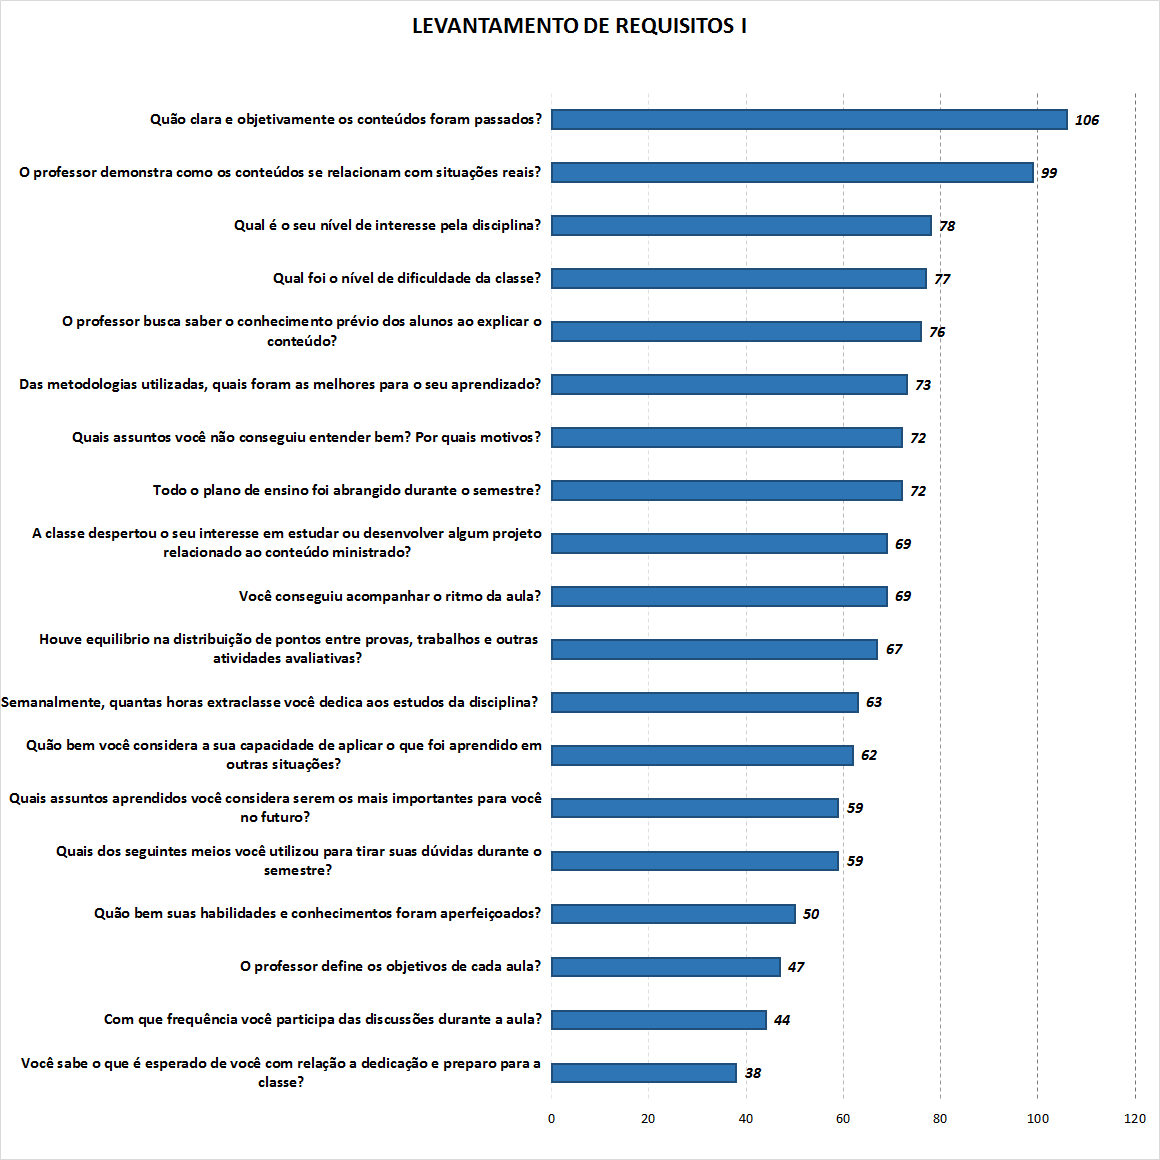
\includegraphics[width=1\textwidth]{img/req_111}
           \subcaption*{Fonte: produzido pelo autor}
        \end{figure}
        
    \newpage
    
    \subsection{Funcionalidades}

    As funcionalidades que o sistema foram definidas separadamente para cada tipo de usuário.

    \newpage
    
    \subsubsection{Aluno}

    A Tabela \ref{tab:funcoes-aluno} apresenta as funções que podem ser executadas pelo usuário do tipo \textit{Aluno}: 

    \begin{table}[h]
    \centering
    \caption{Funcionalidades - Aluno}
    \begin{tabular}{p{5cm} p{10cm}}
    \hline
    Funcionalidade & Descrição \\
    \hline
    \hline
    Responder Questionários & Responder aos questionários atribuídos às suas turmas\\
    \hline
    Visualizar Respostas & Visualização de suas respostas de determinado questionário\\
    \hline
    Visualizar Resultados & Visualização dos resultados de determinado questionário por meio de gráficos de barras\\
    \hline
    Visualizar Turmas & Visualização de detalhes sobre suas turmas atuais e antigas\\
    \hline
    Gerenciar Orientações & Visualização e atualização informações sobre suas orientações\\
    \hline
    Visualizar Professores & Busca e visualização de informações sobre os professores do ICEA (questionários, resultados, turmas, orientações)\\
    \hline
    \end{tabular}
    \caption*{Fonte: produzido pelo autor}
    \label{tab:funcoes-aluno}
    \end{table}
	
    \newpage
    
    \subsubsection{Professor}

    A Tabela \ref{tab:funcoes-prof} apresenta as funcionalidades do \textit{Professor}: 

    \begin{table}[h]
    \centering
    \caption{Funcionalidades - Professor}
    \begin{tabular}{p{5cm} p{10cm}}
    \hline
    Funcionalidade & Descrição \\
    \hline
    \hline      
    Gerenciar Questionários do Professor & Gerenciamento dos questionários criados pelo próprio professor\\
    \hline
    Disponibilizar Questionários do Professor & Disponibilizar questionários criados às turmas do professor\\
    \hline
    Gerenciar Perguntas do Professor & Gerenciamento das perguntas criadas pelo próprio professor\\
    \hline
    Gerenciar Orientações & Criação e atualização de informações sobre suas orientações\\
    \hline
    Visualizar Resultados & Visualização dos resultados de determinado questionário por meio de gráficos de barras\\
    \hline
    Visualizar Alunos & Busca e visualização de informações sobre os alunos do ICEA\\
    \hline
    Visualizar Turmas & Visualizar detalhes sobre suas turmas atuais e antigas\\
    \hline            
    \end{tabular}
    \caption*{Fonte: produzido pelo autor}
    \label{tab:funcoes-prof}
    \end{table}
	
    \newpage 
    
    \subsection{Casos de Uso}

    Casos de uso são comumente utilizados a fim de fazer identificação requisitos de sistemas. \citeonline{pressman:2010} apresenta duas versões dos casos de uso. Eles podem ser simples (pequenas estórias sobre como o usuário interage com o sistema) ou completo (semi-estruturado e com alto nível de detalhamento).  

    Após identificados diferentes tipos de usuários, seus papeis e definidas as principais funcionalidades que eles poderiam executar dentro do sistema, foram criadas versões completas de casos de uso para cada grupo destas funcionalidade seguindo o modelo definido por \citeonline{pressman:2010}. 

    Os casos de uso contribuíram para um melhor entendimento do fluxo de uso do sistema em geral e na identificação de exceções e problemas que poderiam ocorrer durante a utilização do \textit{SisAV}. 
    
    A Figura \ref{fig:usecases_diagram} apresenta o diagrama de casos de uso modelado após a criação dos mesmos:
    
    \begin{figure}[h]	
        \centering
        \caption{Diagrama de Casos de Uso}						   			\label{fig:usecases_diagram}
        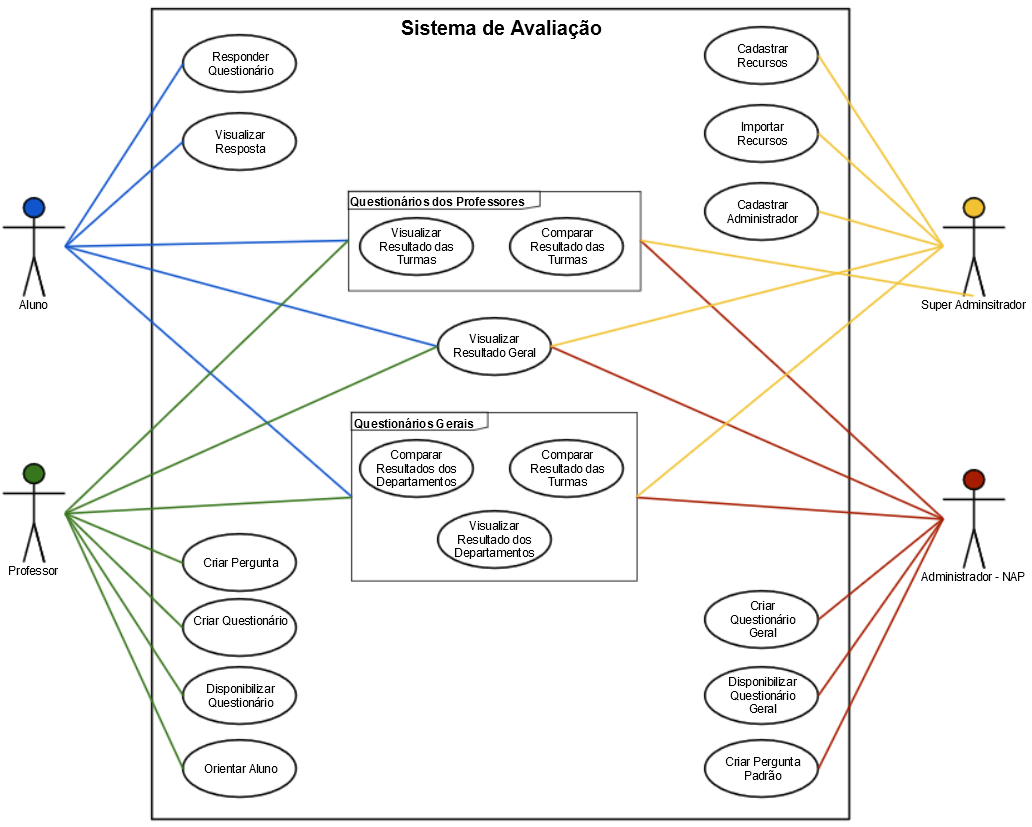
\includegraphics[scale=0.7]{img/usecases_diagram}
        \caption*{Fonte: produzido pelo autor}
    \end{figure}
    
	\subsection{Mapa do Site}
    
    Foram criados quatro mapas de site, correspondendo à cada \textit{homepage} dos usuários do sistema.
    
        \newpage
        
        \subsubsection{Aluno}
		
        A Figura \ref{fig:websitemap_student} apresenta o mapa do site que é acessado pelo \textit{Aluno}:
        
        \begin{figure}[h]	
            \centering
            \caption{Mapa do Site - Aluno}						   \label{fig:websitemap_student}
            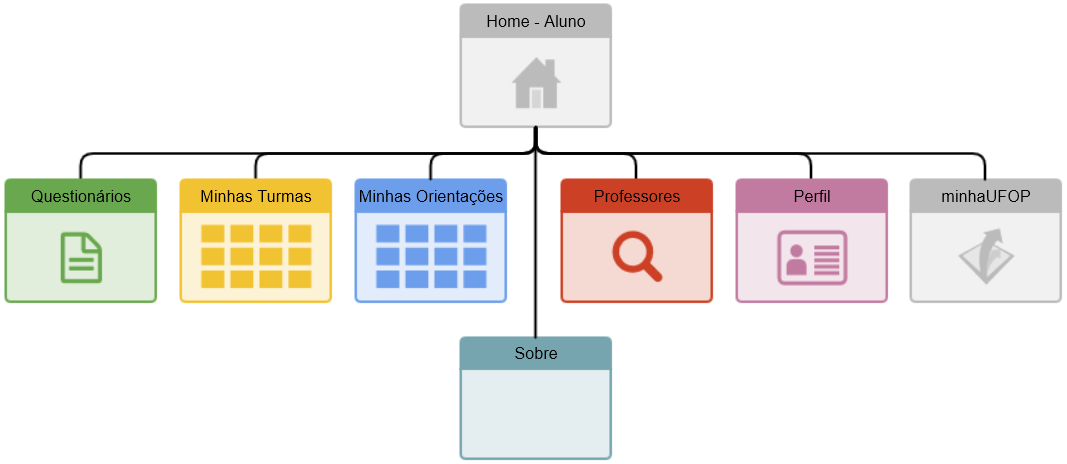
\includegraphics[width=1\textwidth]{img/websitemap_student}
            \caption*{Fonte: produzido pelo autor}
    	\end{figure}
        
        \subsubsection{Professor}
        
        A Figura \ref{fig:websitemap_professor} apresenta o mapa do site que é acessado pelo \textit{Professor}:
		
        \begin{figure}[h]	
            \centering
            \caption{Mapa do Site - Professor}						   \label{fig:websitemap_professor}
            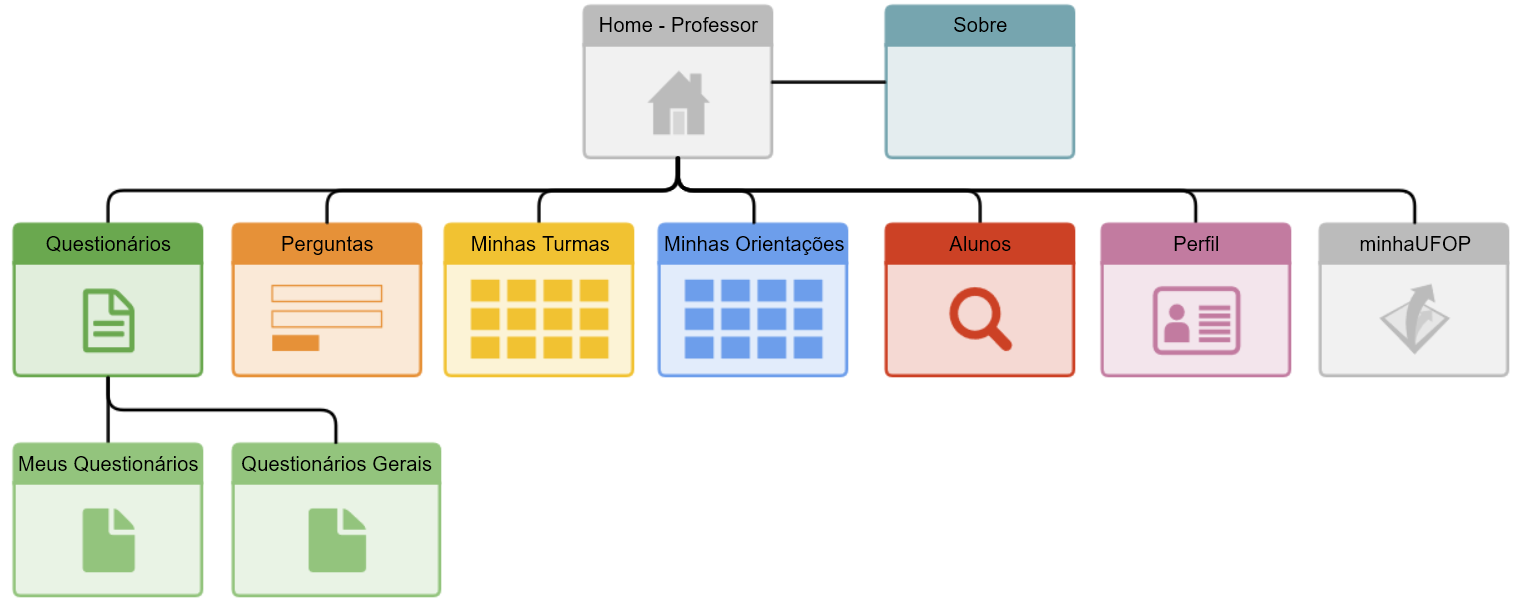
\includegraphics[width=1\textwidth]{img/websitemap_professor1}
            \caption*{Fonte: produzido pelo autor}
    	\end{figure}
    
    \newpage
    
\section{Banco de Dados}

A arquitetura do banco de dados do sistema foi concebida levando em consideração não somente a capacidade do mesmo em atender as atuais necessidades, mas também a facilidade dele em atender futuros requisitos. A seguir é apresentado o Modelo Entidade Relacionamento do banco de dados, o qual foi subdividido em duas partes: \textit{Questionário} e \textit{UFOP}.

	\subsection{Importação de planilhas}

    O banco de dados do sistema veio a ser complexo e robusto. Isso se deu pelo fato do sistema permitir que os usuários criem seus próprios questionários e perguntas. Para garantir este requisito, foi necessário considerar o conjunto de estruturas que compões um questionário (\textit{Perguntas} e seus tipos, \textit{Opções} e \textit{Respostas}) e criar entidades para cada uma delas. A Figura \ref{fig:eer-questionario} mostra como foi modelada a estrutura dos questionários:

    \begin{figure}[h]
        \centering
        \caption{Diagrama EER - Questionários}
        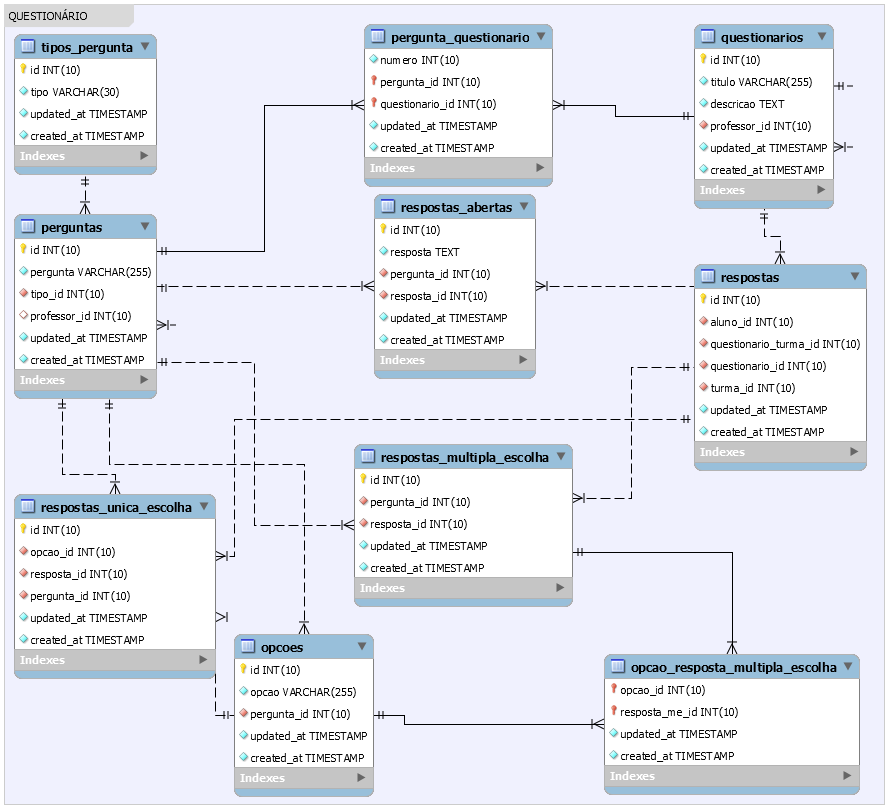
\includegraphics[width=0.8\textwidth]{img/questionario_eer}
        \caption*{Fonte: produzido pelo autor}
        \label{fig:eer-questionario}
    \end{figure}

    \subsection{UFOP}
	
    A Figura \ref{fig:eer-ufop} demonstra a estrutura do banco de dados responsável por armazenar as informações referentes a UFOP:
    
    \begin{figure}[h]
    \centering
    \caption{Diagrama EER - UFOP}
    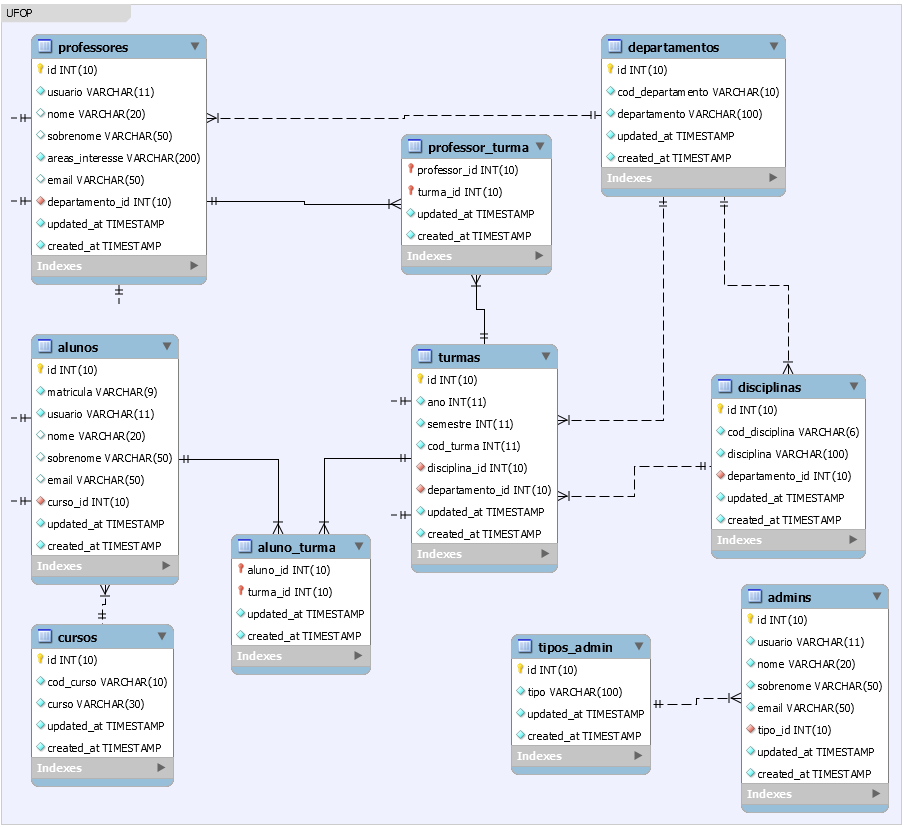
\includegraphics[scale=0.8]{img/ufop_eer}
    \caption*{Fonte: produzido pelo autor}
    \label{fig:eer-ufop}
    \end{figure}

    \section{Desenvolvimento do Sistema}
    
    O desenvolvimento do Sistema de Avaliação foi dividido em quatro etapas. Primeiramente, foi necessário criar a estrutura responsável por processar a autenticação dos usuários da UFOP. Em seguida, foram desenvolvidas as funcionalidade \textit{Create, Read, Update e Delete} (CRUD) para os usuários do tipo \textit{Super Administrador}. Após finalizado o CRUD, foi iniciado o desenvolvimento da funcionalidade principal do sistema, o processamento dos questionários. Por fim, foi iniciada a criação da parte do sistema responsável pelas orientações realizadas na UFOP.
    
        \subsection{Autenticação}

    Um dos pontos observados acerca da autenticação do \textit{SisAV} foi como garantir que somente os usuários permitidos pudessem acessar a plataforma. Caso o cadastros de usuários fosse necessário, verificar se o usuário recém-cadastrado pertence a UFOP seria bastante inviável. Com o propósito de contornar esta situação indesejável e facilitar o acesso para os usuários, foi determinado que a autenticação do sistema deveria ser feita a partir das credenciais previamente cadastradas na UFOP, sendo as mesmas que os discentes e docentes utilizam para acessar o portal \textit{minhaUFOP}.

    Antes de começar o desenvolvimento do módulo responsável pela autenticação, o orientador Theo Silva Lins requisitou as credenciais necessárias para acessar o \textit{OpenLDAP} da UFOP. Estas, por sua vez, foram fornecidas pelo NTI do campus de Ouro Preto. O usuário utilizado para acessar a base de dados da UFOP possui apenas permissões para leitura, evitando que qualquer tipo de problema pudesse ocorrer ao utilizar o \textit{OpenLDAP}.

    Com o objetivo de entender melhor a estruturação do \textit{OpenLDAP} da UFOP, foi utilizado o software \textit{Apache Directory Studio}\footnote{http://directory.apache.org/studio/}. Ele permitiu a visualização e estudo de todas a estruturas das DITs do \textit{OpenLDAP}. A partir desta análise, foram identificadas as informações necessárias para o sistema e os nomes dos campos onde elas são armazenadas.
    
    Os registros pertencentes à unidade organizacional \textit{People}, possuem um campo denominado \textit{ou}, o qual corresponde a um registro da unidade organizacional \textit{Grupos}. O usuário apenas tem acesso ao sistema caso suas credenciais estejam corretas e se o valor do campo \textit{ou} esteja pré-cadastrados no banco de dados do \textit{SisAV}. 

    Após o usuário ser autenticado pela primeira vez no sistema, suas informações (senha não inclusa) são armazenadas na base de dados. Nas próximas autenticações, as informações armazenadas apenas serão comparadas com aquelas do \textit{OpenLDAP} e, caso necessário, a atualização da base de dados do sistema é realizada.

        \subsection{CRUD dos Registros}

    O CRUD dos registros tais como departamentos, disciplinas, turmas, ajustes de matrícula, discentes, docentes e administradores, são operações exclusivas dos usuários do tipo \textit{Super Administrador}. 

    Informações básicas (departamentos, cursos, disciplinas, tipos de administrador) são gerenciadas a partir de formulários HTML ordinários. Cada uma destas informações são consideradas uma entidade do banco de dados, possuindo seus respectivos \textit{Controllers} e \textit{Models}. As operações CRUD destas entidades foram desenvolvidas de forma padronizada, existindo apenas alteração nos atributos manipulados. As permissões de acesso dos discentes e docentes são gerenciadas a partir dos departamentos e cursos cadastrados na base de dados, ou seja, apenas docentes dos departamentos existentes e discentes dos cursos existentes conseguem acessar o \textit{SisAV}.     

    Registros referentes aos docentes, discentes, turmas, e ajustes de matrículas foram adicionados a base de dados do sistema a partir de arquivos \textit{.CSV} disponibilizados pela seção de ensino do ICEA. Uma vez que não foi possível termos acesso direto ao banco de dados da UFOP durante o desenvolvimento do trabalho, foi necessário criar funções específicas para fazer a importação destas informações. Apenas arquivos do tipo \textit{.CSV} são aceitos e estes devem ser padronizados conforme o formato gerado pela seção de ensino.

    Os administradores do sistema devem estar pré-cadastrados na base de dados para que eles acessem o sistema. Assim, foi desenvolvido o CRUD dos administradores, onde é necessário que o usuário defina além das informações pessoais, o tipo do administrador (Super Administrador, Administrador - NAP) que ele está criando. 

        \subsection{Processo de gerenciamento de faltas}

    	O desenvolvimento das funções relativas aos questionários foi subdividido e realizado na seguinte ordem: criação e disponibilização, resposta e visualização dos resultados.

            \subsubsection{Criação e Disponibilização}

            A criação dos questionários, independentemente dele ser geral ou de um professor, é feita exatamente da mesma maneira e o processo é completamente dinâmico. Para isso, foram utilizados \textit{JQuery} e \textit{Ajax}, permitindo que o usuário não somente adicione e remova perguntas previamente criadas, mas também que ele crie novas perguntas no momento, definindo o tipo e as opções das mesmas. Com o objetivo de acomodar a necessidade da existência de questionários gerais para a UFOP, foi decidido utilizar a técnica chamada \textit{Single Table Inheritance}. Esta prática é um dos modos de simular uma herança da orientação de objetos em um banco de dados relacional. Assim, antes do questionário ser inserido no banco de dados, é verificado o tipo do usuário que o criou e, caso o usuário que fez a requisição seja do tipo \textit{Administrador - NAP}, a chave estrangeira \textit{professor\_id} recebe o valor \textit{NULL}. Caso contrário, ela simplesmente recebe o valor do \textit{ID} do professor. O valor nulo representa a inexistência do proprietário do questionário, o que por sua vez significa que este poderá ser distribuído à todas turmas da UFOP.

            A mesma metodologia foi empregada para tratar as perguntas dos questionários. Se uma pergunta possui o \textit{ID} de um professor, a mesma só poderá ser adicionada aos questionários que este criar. Caso contrário, a chave estrangeira será nula, indicando que apenas os administradores poderão adicioná-las aos questionários gerais criados por eles.

            \subsubsection{Acesso as faltas e solicitação de abono}

            Quando docentes ou o NAP disponibilizam os questionários às turmas, os discentes destas turmas, podem acessar o mesmo e respondê-lo. O formulário de respostas é construído após ser feita a requisição para responder o questionário. O \textit{Controller} dos questionários é responsável por buscar o questionário, as perguntas pertencentes ao mesmo e as opções destas perguntas. O tipo de \textit{input} a ser gerado depende do tipo da pergunta. Elas podem ser abertas (\textit{text input}), fechadas - única escolha (\textit{radio}) e fechadas - múltipla escolha (\textit{checkbox}). A relação entre perguntas e questionários possui um atributo \textit{numero} que é utilizado para garantir que as perguntas sejam exibidas na mesma ordem em que elas foram adicionadas ao questionários. Além do formulário para respostas, também são exibidos o título e descrição do questionário para que os discentes que o forem responder entendam o objetivo do mesmo. 
            
            A visualização das respostas de um discente é uma funcionalidade restrita somente aos administradores do sistema ou ao próprio discente. Os docentes não possuem acesso as respostas específicas de um discente, já que é necessário manter o anonimato dos mesmos para os docentes.

            \subsubsection{Visualização das Aprovações de Abono}

			A visualização dos resultados é um funcionalidade universal, podendo ser utilizada por qualquer usuário autenticado no sistema. No entanto, existem restrições sobre a exibição do resultado de acordo com o tipo do usuário que o está acessando. O resultado das questões fechadas pode ser visualizado por qualquer tipo de usuário. Todavia, as respostas das questões abertas podem ser acessadas apenas por administradores e pelo docente que disponibilizou determinado questionário. Esta restrição teve que ser imposta já que, ao contrário de perguntas fechadas, não é possível controlar o que cada discente escreverá nas perguntas abertas.

            Para exibir o resultado das perguntas fechadas, foi utilizado o \textit{Chart.js}\footnote{http://www.chartjs.org/}. Este é uma biblioteca desenvolvida em \textit{Javascript} para criação de diversos tipos de gráficos responsivos. Foi utilizado o gráfico de barra vertical gerado pelo \textit{Chart.js}. 

			A porcentagem de escolhas das opções é dada pela seguinte fórmula: 
            
            $$\frac{\sum R * P_{i}}{100}$$
            
            onde $R$ é o número total de respostas (número de alunos que responderam o questionário) e $P_{i}$ é o número de escolhas da opção $i$ da pergunta $P$. É importante destacar que para as perguntas que permitem uma única escolha, a soma das porcentagens das escolhas resultada em cem porcento, enquanto que para as perguntas que permitem que os alunos escolham mais de uma opção, isto não será verdade.
            
            O usuário pode visualizar o resultados dos questionários de três maneiras:

            \begin{enumerate}

            \item \textbf{Resultado Geral}: o resultado geral processa as respostas de todas as turmas em que determinado questionário foi disponibilizado. A Figura \ref{fig:resultado_geral} mostra a consolidação de resultados gerados aleatoriamente para as turmas que responderam o questionário \textit{Pesquisa de Desenvolvimento de Disciplinas da Graduação da UFOP}:
            
            \begin{figure}[h]
                \centering
                \caption{Tela - Resultado Geral}
                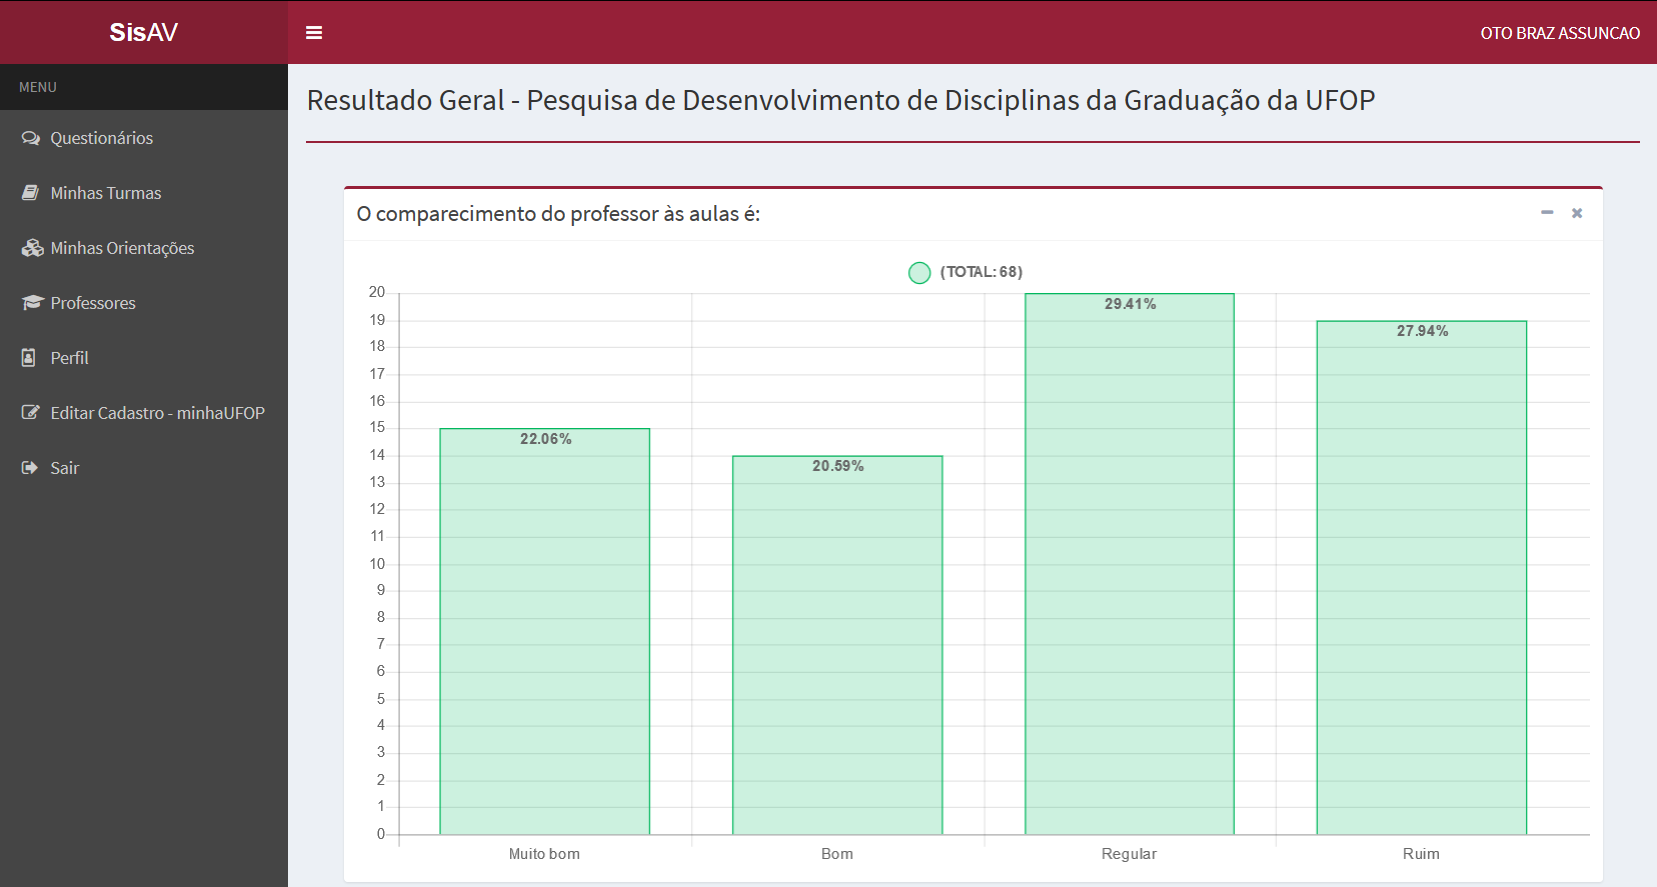
\includegraphics[width=1\textwidth]{img/resultado_geral}
                \caption*{Fonte: produzido pelo autor}
                \label{fig:resultado_geral}
   		 	\end{figure}

            \item \textbf{Resultado Específico}: a maneira como estes estes são gerados é dependente do tipo do questionário. Os resultados específicos dos questionários dos professores são baseados nas turmas, mostrando o resultado da turma escolhida. Os resultado específico dos questionários gerais, por sua vez, são baseados nos departamentos, exibindo o resultado do departamento desejado. A Figura \ref{fig:resultado_especifico} exemplifica o resultado gerado aleatoriamente para a classe Projeto e Análise de Algoritmo - Turma 11:
            
            \newpage
            
            \begin{figure}[h]
                \centering
                \caption{Tela - Resultado Específico}
                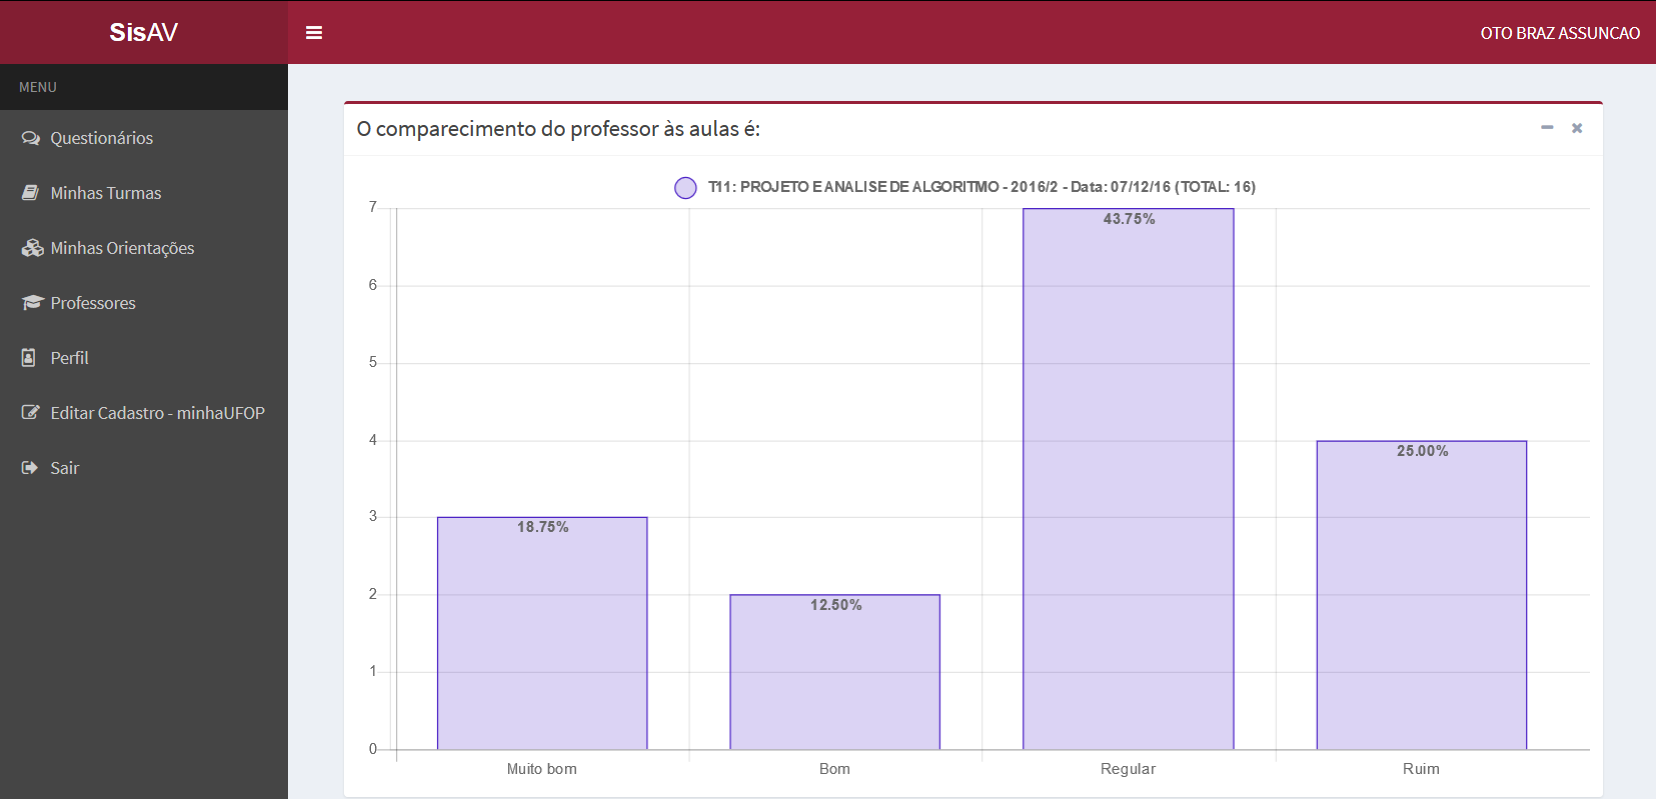
\includegraphics[width=1.0\textwidth]{img/resultado_especifico}
                \caption*{Fonte: produzido pelo autor}
                \label{fig:resultado_especifico}
   		 	\end{figure}

            \item \textbf{Resultados Comparados}: os questionários dos professores permitem que o usuário faça a comparação dos resultados entre as turmas daquele professor que responderam o questionário, enquanto que os questionários gerais proporcionam não somente a comparação entre as turmas, mas também entre os departamentos. A Figura \ref{fig:resultado_comparados} apresenta um exemplo da comparação de resultados aleatórios da \textit{Turma 11 - Compiladores I} e da \textit{Turma 11 - Projeto e Análise de Algoritmos}:
            
            \begin{figure}[h]
                \centering
                \caption{Tela - Resultados Comparados}
                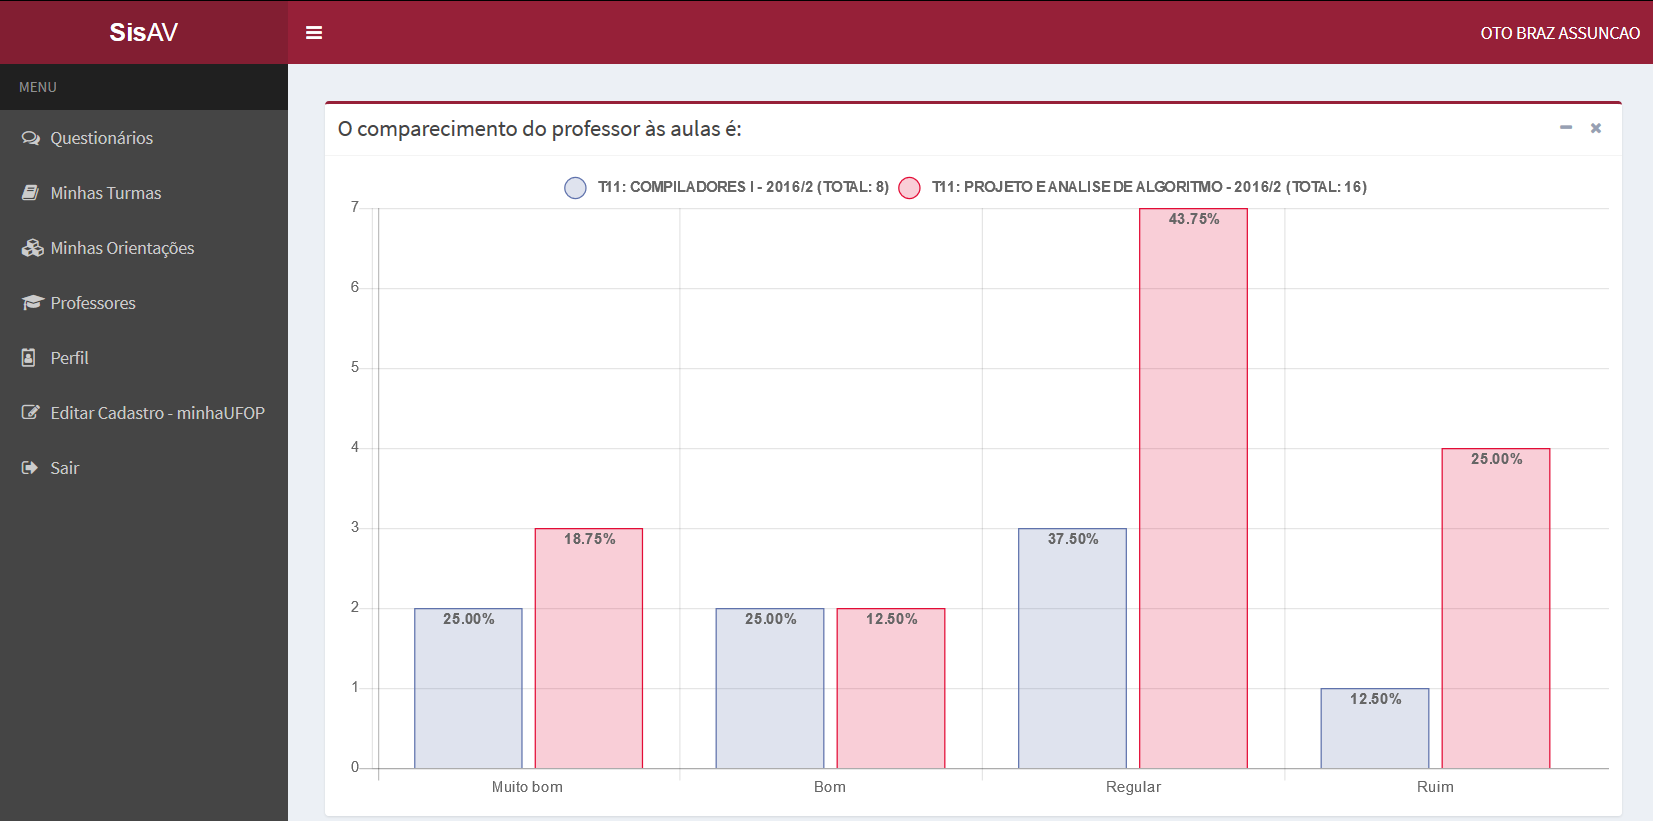
\includegraphics[width=1\textwidth]{img/resultados_comparados}
                \caption*{Fonte: produzido pelo autor}
                \label{fig:resultado_comparados}
   		 	\end{figure}

    		\end{enumerate}

        \subsection{Tutorial }
       
		Após finalizadas todas as funcionalidades dos questionários, foi dado início a parte da aplicação responsável pelo gerenciamento das orientações da UFOP. Primeiramente, a busca pelos \textit{Alunos} e capacidade de iniciar uma orientação foi adicionada para o \textit{Professor} conforme exemplificado pela Figura \ref{fig:alunos_home}: 
        
        \begin{figure}[h]
        \centering
        \caption{Tela - Busca pelos Alunos}
        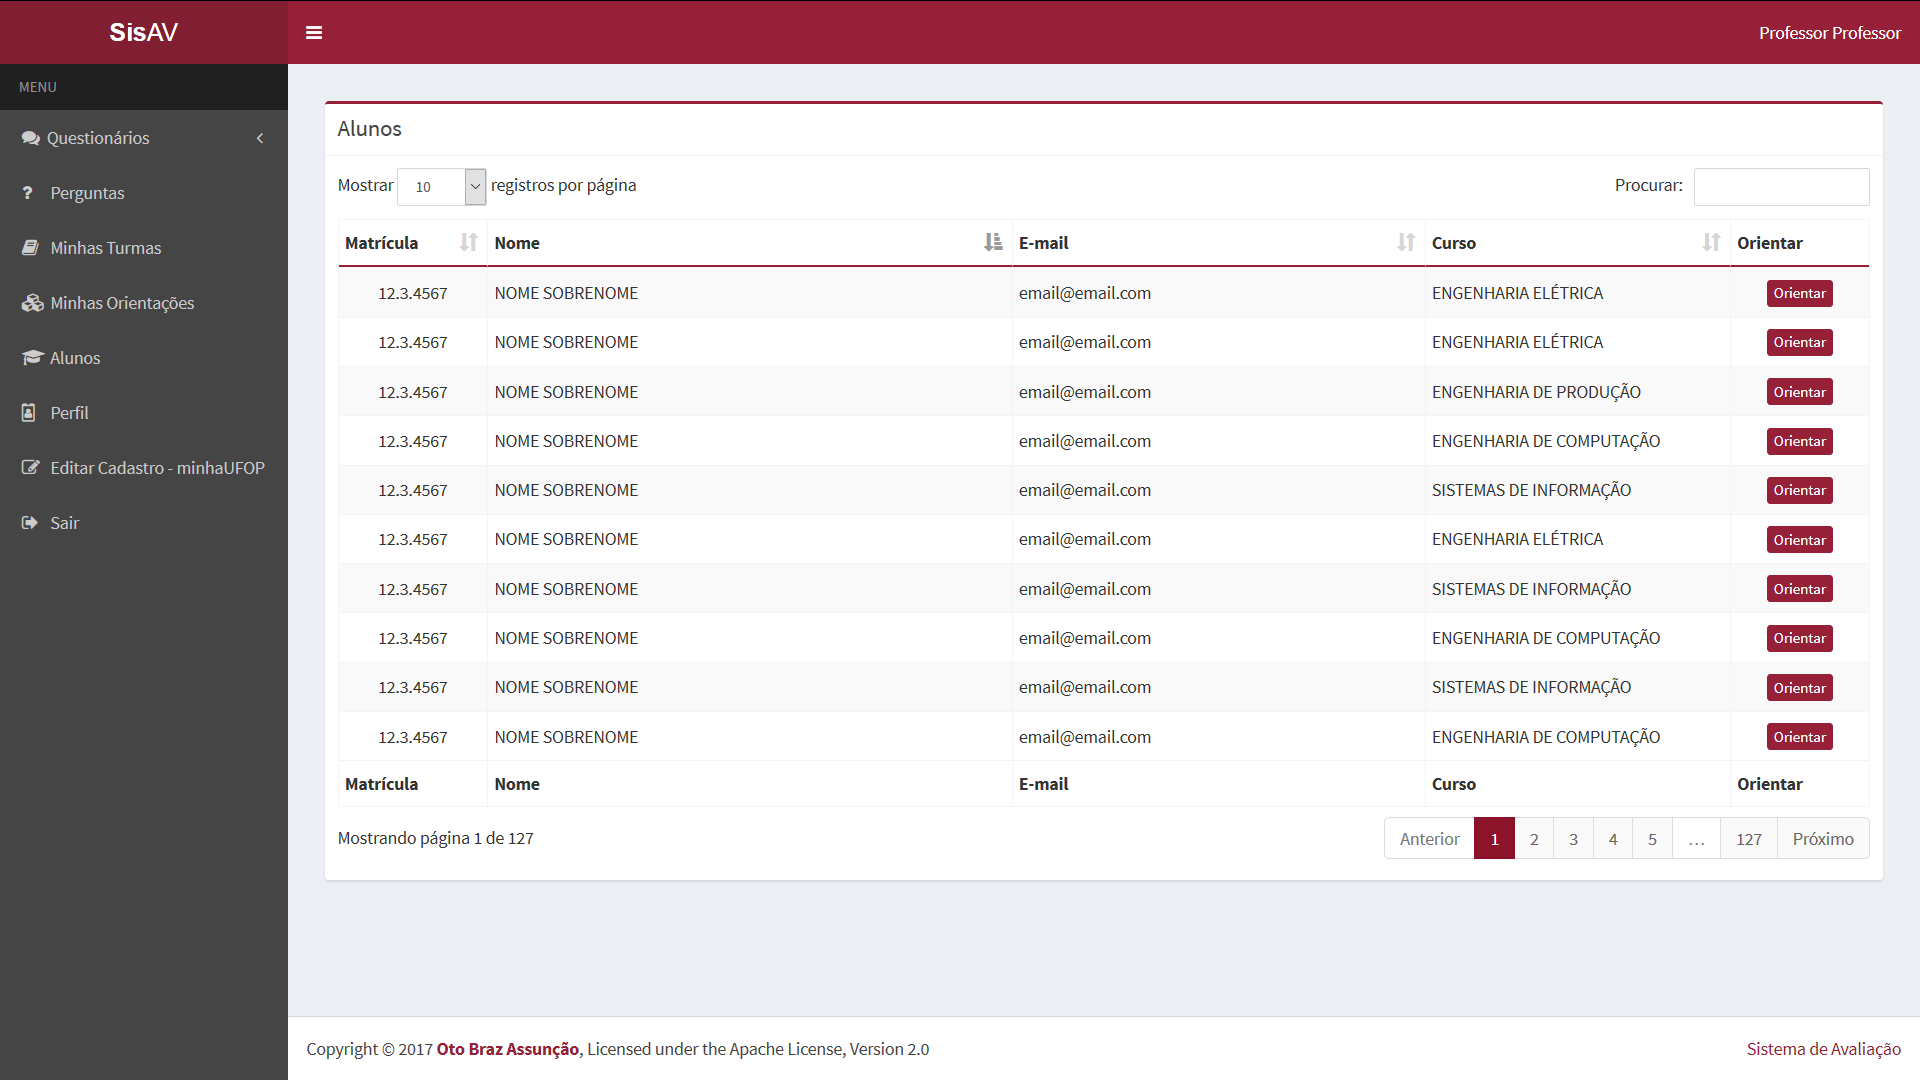
\includegraphics[width=0.8\textwidth]{img/alunos_home}
        \caption*{Fonte: produzido pelo autor}
        \label{fig:alunos_home}
        \end{figure}
		
        Em seguida, foram desenvolvidas as funcionalidades de gerenciamento, que podem ser feitas tanto pelo \textit{Professor} que criou a orientação (Figura \ref{fig:orientacoes_home}) quanto pelo \textit{Aluno} orientado.
        
        \begin{figure}[h]
        \centering
        \caption{Tela - Orientações (\textit{Professor)}}
        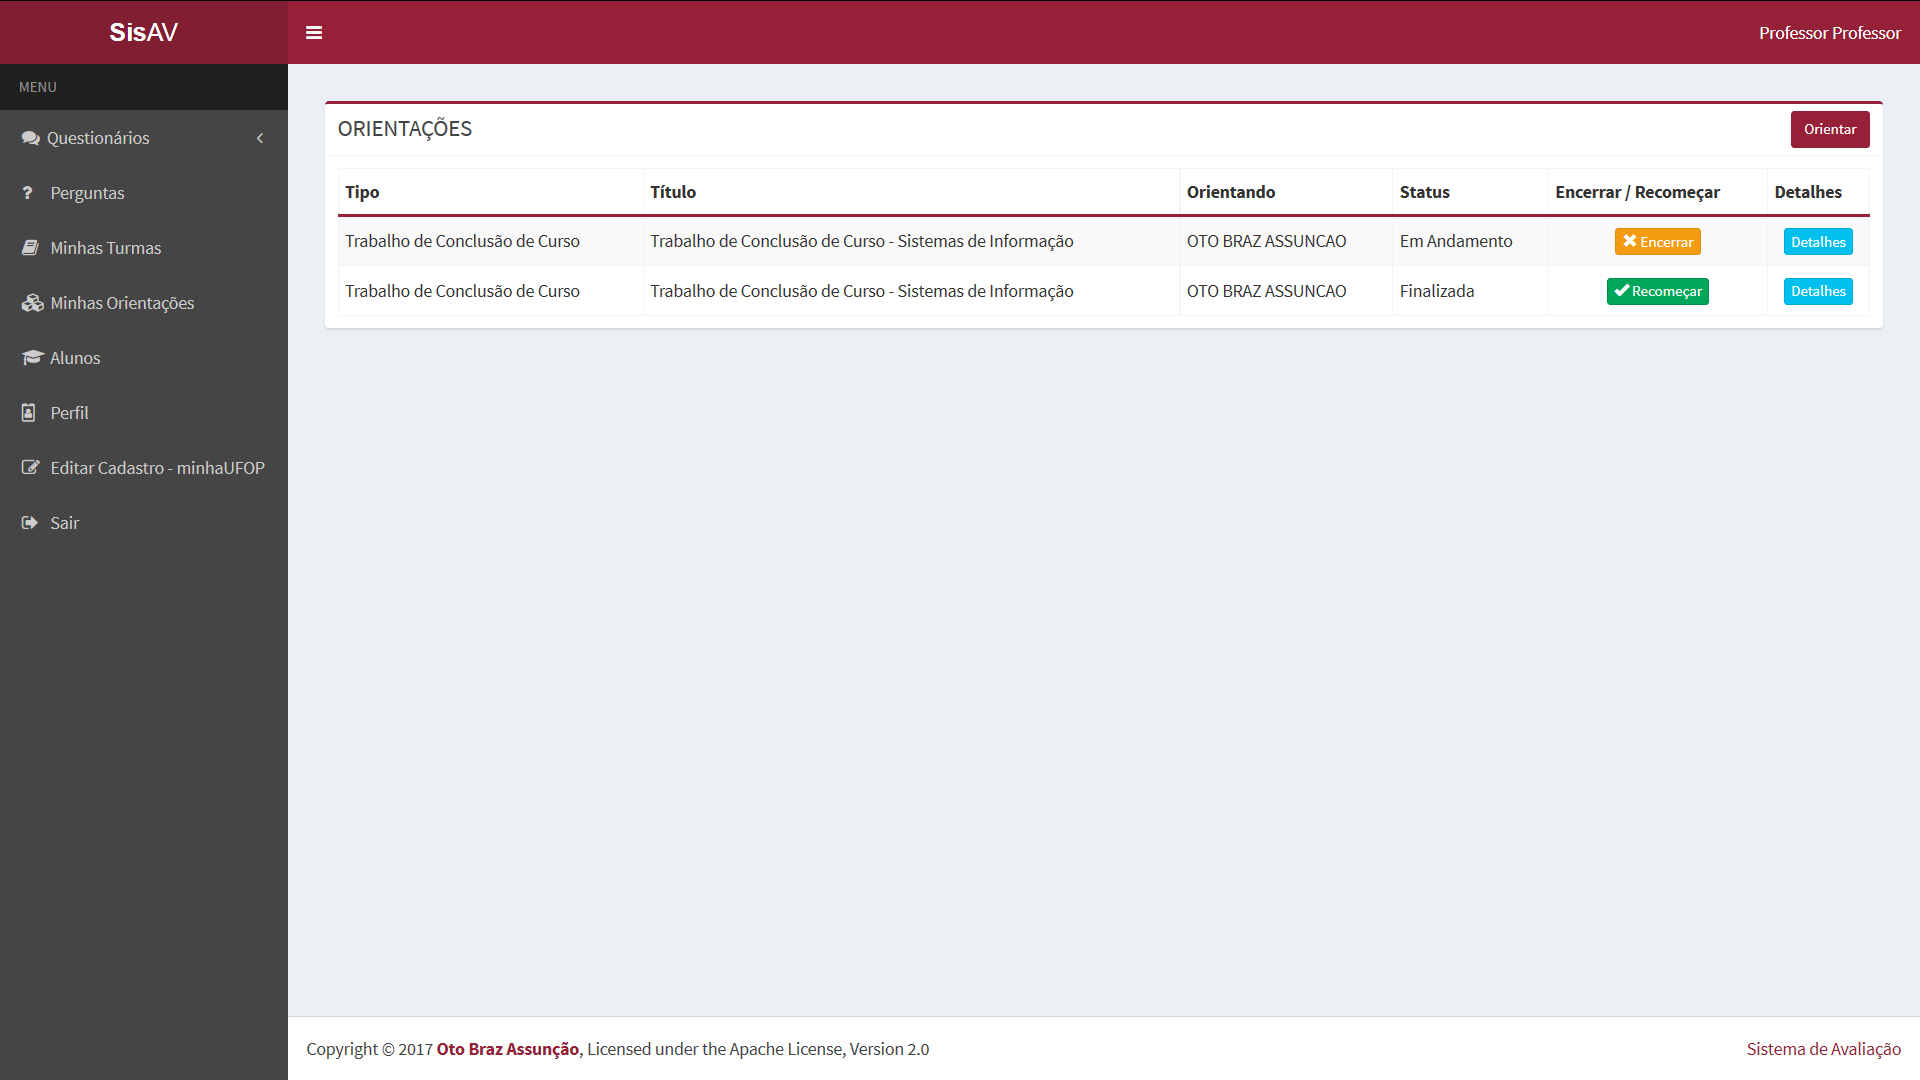
\includegraphics[width=0.8\textwidth]{img/orientacoes_home1}
        \caption*{Fonte: produzido pelo autor}
        \label{fig:orientacoes_home}
        \end{figure}
        
        \subsection{Testes automatizados com o Framework Selenium}

        Foram executados basicamente dois tipos de testes de desenvolvimento: \textit{teste em ambiente de desenvolvimento} e \textit{teste em ambiente de produção}. O teste de desenvolvimento é o tipo de teste realizado durante a fase de produção do sistema pelos desenvolvedores com o objetivo de identificar \textit{bugs}, erros e não-conformidades \cite[p. 210]{sommervile:2011}.

           Foi feita a utilização da biblioteca \textit{Faker} \footnote{https://github.com/fzaninotto/Faker} para adição de dados de teste ao banco de dados do sistema. A princípio, foram gerados dados aleatórios para todas as tabelas do banco de dados já que não foi possível acessar às informações reais da UFOP. Conforme o acesso as informações reais foi obtido, as mesmas foram sendo adicionadas à base de dados e os dados de teste removidos. Por fim, os únicos dados de teste que restaram no sistema foram aqueles referentes aos questionários dos \textit{Professores} e as respostas aleatórias dos \textit{Alunos}. 
       
			\subsubsection{Testes em Ambiente de Desenvolvimento}

			Sempre que uma nova funcionalidade foi desenvolvida, independentemente da complexidade da mesma, ela foi testada individualmente no ambiente de desenvolvimento. Após atestado que ela funcionou conforme o esperado, foram executados testes das demais funcionalidades que estavam relacionadas àquela recém-desenvolvida.
           
			\subsubsection{Testes em Ambientes de Produção}
       
       		Quando o desenvolvimento chegou a um ponto em que o sistema pudesse ser utilizado, mesmo com limitações, pelos usuários, foi feita hospedagem do \textit{website} em um servidor online a fim de serem executados os testes em ambiente de produção. O sistema no ambiente de produção foi atualizado à medida que foram feitos o desenvolvimento e teste de um conjunto de funcionalidades no ambiente de desenvolvimento.
            
            O principal problema identificado durante os testes do \textit{website}, foi a diferença na maneira em que \textit{MariaDB} (ambiente de desenvolvimento) e o \textit{MySQL} (ambiente de produção) tratavam os números. As consultas realizadas no \textit{MariaDB} retornavam os números exatamente como \textit{Integers}, enquanto que aquelas feitas no \textit{MySQL} retornavam os números como \textit{Strings}. Devido a esta diferença, algumas partes do sistema online deixaram de funcionar já todos os números estavam sendo manipulados como \textit{Integers}.
                               
	%\section{Reunião com o NAP e Validação do Sistema}

	Após a produção do sistema ter atingido o seu estágio final, foi agendada uma reunião com o NAP da UFOP para apresentação do projeto desenvolvido e obtenção de \textit{feedbacks} e sugestões. Participaram da reunião o Adilson Pereira dos Santos e Mônica Versiani Machado do NAP, Theo Silva Lins, orientador, e Oto Braz Assunção, orientando. 
    
    Primeiramente o projeto foi apresentado ao NAP, as motivações, como ele poderia beneficiar a UFOP e tudo aquilo que tinha sido desenvolvido até o momento da reunião. A situação atual da UFOP também foi discutida e foi reconhecido que a PDDGU está ultrapassada e que este projeto poderá, junto com a PDDGU, contribuir para constante melhora do ensino fornecido pela UFOP.
    
    Além da possibilidade dos professores gerenciar seus próprios questionários, foi definido na reunião que permitir a criação e disponibilização de um questionário geral para todo o campus seria fundamental para o NAP. Eles não possuem muito controle sob a PDDGU, fazendo apenas uma requisição ao NTI quanto a data de liberação da pesquisa nos semestres. Assim, foi dada permissão de acesso ao sistema ao grupo de usuários pertencentes ao NAP e a capacidade deles gerenciarem completamente os questionários gerais. 
    
    É esperado que o Sistema de Avaliação seja implantado no ICEA como projeto-piloto no primeiro semestre de 2017. A intenção do NAP é utilizar a plataforma para disponibilizar os questionários gerais durante o início e o meio de cada semestre letivo. O projeto-piloto no ICEA será conduzido através do programa Pró-Ativa, em que o discente responsável, juntamente com o orientador Theo Silva Lins, gerenciará o processo de implantação. Os principais objetivos do projeto-piloto serão a obtenção de \textit{feedback} do corpo discente e docente do campus e adaptação do \textit{SisAV} caso seja necessário. 
    
% ---

\chapter{Considerações Finais}\label{conclusao}
% ---
    
O desenvolvimento deste trabalho demonstrou ser um processo muito mais complexo do que o esperado uma vez que garantir que sistema atenda à todas as necessidades da UFOP não é algo simples. 

Houve a dificuldade de conseguir um grau alto de participação do corpo discente e docente nos questionários aplicadas durante o processo de identificação dos requisitos e planejamento do sistema. Ademais, não foi possível realizar a reunião com o NAP durante as etapas iniciais do projeto, o que acabou levando a alteração de requisitos no estágio final do desenvolvimento. Logo, a etapa de implantação foi adiada e foi dada prioridade a conformidade com as novas necessidades identificadas e adaptação do sistema para que o discente responsável pela implantação do \textit{SisAV} se familiarize facilmente com o sistema produzido.

No decorrer de todo o projeto foram realizadas reuniões semanais com os orientadores do mesmo a fim de discutir o andamento do trabalho, problemas enfrentados e definir tarefas a serem executadas e a prioridade de cada uma delas. Deste modo, foi possível garantir que o projeto evoluísse constantemente em todas as etapas. Durante as reuniões, novos requisitos foram definidos e alguns dos existentes adaptados. A utilização do \textit{framework} MVC \textit{Laravel} foi um dos fatores primordiais que contribuíram para a diminuição da complexidade de adaptação do sistema aos novos requisitos.

A versão atual do \textit{SisAV} requer que os usuários do tipo \textit{Administrador - NAP} disponibilizem e encerrem manualmente os questionários gerais em cada semestre. Ainda não é possível fazer a exportação dos resultados de ambos os questionários gerais e questionários do professor. Por fim, a importação das informações contidas nos arquivos \textit{.CSV} disponibilizados pela seção de ensino é sempre necessária ao início de cada semestre. 

Espera-se que as limitações do sistema sejam resolvidas durante o projeto-piloto e que, após a finalização do mesmo, o \textit{SisAV} seja implantando em toda instituição e utilizado, juntamente com a PDDGU, para afetar positivamente a qualidade do ensino oferecida pela UFOP.
    
% ---

%\chapter{Limitações e Trabalhos Futuros}\label{limitacoes}
% ---



%A fim de tornar o processo de disponibilização e encerramento mais eficiente, a adição de uma funcionalidade para permitir que os usuários definam previamente as datas de disponibilização e encerramento será adicionada. Assim, com exceção da definição das datas, todo o processo será realizado automaticamente.

%Exportar os resultados para arquivos \textit{PDF} e \textit{CSV} é algo que facilitaria o acesso aos mesmos em ambientes onde o acesso ao sistema não pode ser realizado.

%Por fim, a importação das informações contidas nos arquivos \textit{.csv} disponibilizados pela seção de ensino é sempre necessária ao início de cada semestre. Quando a permissão de acesso a base de dados da UFOP for concedida, espera-se obter estas informações diretamente deste banco de dados. Assim, o processo de importação será desnecessário no futuro.

% Embora as limitações acima citadas tenham sido reconhecidas, não foi possível contorná-las. A intenção é que as mesmas sejam contornadas no próximo semestre, fazendo com que o Sistema de Avaliação possua um grau de usabilidade ainda maior.  

% ----------------------------------------------------------
% Finaliza a parte no bookmark do PDF
% para que se inicie o bookmark na raiz
% e adiciona espaço de parte no Sumário
% ----------------------------------------------------------
\phantompart

% ---
% Conclusão (outro exemplo de capítulo sem numeração e presente no sumário)
% ---
% \chapter*[Conclusão]{Conclusão}
% \addcontentsline{toc}{chapter}{Conclusão}
% % ---

% \lipsum[31-33]

% ----------------------------------------------------------
% ELEMENTOS PÓS-TEXTUAIS
% ----------------------------------------------------------
\postextual
% ----------------------------------------------------------

% ----------------------------------------------------------
% Referências bibliográficas
% ----------------------------------------------------------
\bibliography{abntex2-modelo-references}
\nocite{gosling:2005,smith:99}

% ----------------------------------------------------------
% Glossário
% ----------------------------------------------------------
%
% Consulte o manual da classe abntex2 para orientações sobre o glossário.
%
%\glossary

% ----------------------------------------------------------
% Apêndices
% ----------------------------------------------------------

% ---
% Inicia os apêndices
% ---
\begin{apendicesenv}

% Imprime uma página indicando o início dos apêndices
\partapendices

\setlength{\parindent}{0in}

% ----------------------------------------------------------
\chapter{Questionário - Pesquisa de Desenvolvimento de Disciplinas da Graduação da UFOP (respondida pelos discentes)}\label{questionario_1}
% ----------------------------------------------------------

		\textit{Esse questionário tem como objetivo saber a opinião dos professores sobre a pesquisa da PROGRAD a fim de levantar requisitos para o Trabalho de Conclusão de Curso sendo desenvolvido por mim, Oto Braz Assunção, aluno do curso de Sistemas de Informação. O trabalho consiste na criação de uma plataforma web para que os alunos compartilhem suas opiniões a respeito das aulas assistidas e orientações recebidas. A partir das respostas, o sistema proverá um feedback que pode ser utilizado tanto pelos professores quanto alunos. Desta maneira, os alunos poderão saber o que esperar das aulas e os professores saberão, eficientemente, quais aspectos eles podem aprimorar a fim de melhorar a qualidade do ensino e orientações.}
        
        \textbf{1. Você sabe qual o objetivo da pesquisa?}
        	
            \begin{itemize}[label=\Circle]             
            \item Sim
            \item Não                   
            \end{itemize}
        
        \textbf{2. Como você costuma receber os resultados da pesquisa?}
        
        \_\_\_\_\_\_\_\_\_\_\_\_\_\_\_\_\_\_\_\_\_\_\_\_\_\_\_\_\_\_\_\_\_\_\_\_\_\_\_\_\_\_\_\_\_\_\\
        
        \textbf{3. A divulgação dos resultados é:}
        
        PÉSSIMA - \Circle 1 \Circle 2 \Circle 3 \Circle 4 \Circle 5 - ÓTIMA\\
        
        \textbf{4. A forma como os resultados são apresentados é:}
        
        PÉSSIMA - \Circle 1 \Circle 2 \Circle 3 \Circle 4 \Circle 5 - ÓTIMA\\
        
        \textbf{5. Você faz a análise dos resultados das pesquisas?}
        
            \begin{itemize}[label=\Circle]            
            \item Sim
            \item Não                  
            \end{itemize}
        
        \textbf{6. A conveniência ao buscar pelos resultados de pesquisas anteriores é:}
        
        PÉSSIMA - \Circle 1 \Circle 2 \Circle 3 \Circle 4 \Circle 5 - ÓTIMA\\
        
        \textbf{7. O número de vezes que a pesquisa lhe ajudou a melhorar o ensino foi:}
        
        MUITO BAIXA - \Circle 1 \Circle 2 \Circle 3 \Circle 4 \Circle 5 - MUITO ALTA\\
        
        \textbf{8. Você considera que os tópicos abordados na pesquisa são o suficiente?}
        
            \begin{itemize}[label=\Circle]           
            \item Sim
            \item Não                  
            \end{itemize}
        
        \textbf{9. Você considera que as notas influenciam as respostas dos alunos?}
        
            \begin{itemize}[label=\Circle]        
            \item Sim
            \item Não       
            \end{itemize}
        
        \textbf{10. Em geral, você considera que a eficiência da pesquisa é?}
        
        MUITO BAIXA - \Circle 1 \Circle 2 \Circle 3 \Circle 4 \Circle 5 - MUITO ALTA\\
        
        \textbf{11. Você considera que pesquisas do tipo devam ser realizadas durante:}
        	
            \begin{itemize}[label=\Circle]
            
            \item Apenas no fim do semestre
            \item Início e Fim do semestre
            \item Início, meio e fim do semestre
            
            \end{itemize}
        
        \textbf{12. Quais você considera serem as principais limitações da atual pesquisa?}
        	
            \begin{multicols}{2}
            \begin{itemize}[label=\Square]       
            \item Número de questões          
            \item Tópicos abordados         
            \item Época que a pesquisa é realizada           
            \item Tempo levado para divulgação dos resultados           
            \item Influência de fatores irrelevantes nas respostas dos alunos            
            \item Falta de questões abertas            
            \item Nível de detalhamento
            \item Other: \_\_\_\_\_\_\_\_\_\_\_\_\_\_\_\_\_\_\_\_\_\_           
            \end{itemize}
            \end{multicols}

% ----------------------------------------------------------
\chapter{Questionário - Levantamento de Requisitos I}\label{questionario_2}
% ----------------------------------------------------------

  	\textit{Esse questionário tem como objetivo levantar requisitos para o meu Trabalho de Conclusão de Curso. O trabalho consiste na criação de uma plataforma web para que os alunos compartilhem suas opiniões a respeito das aulas e orientações que receberam de professores. A partir das respostas, o sistema proverá um feedback que pode ser utilizado tanto pelos professores quanto alunos. Deste modo, os alunos poderão saber o que esperar das aulas e os professores saberão, eficientemente, quais aspectos eles podem aprimorar a fim de melhorar a qualidade do ensino e orientações.}
  
  	\textbf{1. Dentre as opções abaixo, escolha aquelas que você considera mais importantes a serem abordadas no questionário sobre as aulas:}
    
    \begin{itemize}[label=\Square]
        \item Todo o plano de ensino foi abrangido durante o semestre?
        \item Quão clara e objetivamente os conteúdos foram passados?
        \item O professor define os objetivos de cada aula?
        \item O professor demonstra como os conteúdos se relacionam com situações reais?
        \item O professor busca saber o conhecimento prévio dos alunos ao explicar o conteúdo?
        \item Das metodologias utilizadas, quais foram as melhores para o seu aprendizado?
        \item Houve equilíbrio na distribuição de pontos entre provas, trabalhos e outras atividades avaliativas?
        \item  Você sabe o que é esperado de você com relação a dedicação e preparo para a classe?
        \item Semanalmente, quantas horas extraclasse você dedica à classe?
        \item Com que frequência você participa das discussões durante a aula?
        \item Qual foi o nível de dificuldade da classe?
        \item Você conseguiu acompanhar o ritmo da aula?
        \item Quais assuntos você não conseguiu entender bem? Por quais motivos?
        \item Quais dos seguintes meios você utilizou para tirar suas dúvidas durante o semestre?
        \item Quão bem suas habilidades e conhecimentos foram aperfeiçoados?
        \item Quão bem você considera a sua capacidade de aplicar o que foi aprendido em outras situações?
        \item Quais assuntos aprendidos você considera serem os mais importantes para você no futuro?
        \item Qual é o seu nível de interesse pela disciplina?
        \item A classe despertou o seu interesse em estudar ou desenvolver algum projeto relacionado ao conteúdo ministrado?
    \end{itemize}
  
  	\textbf{2. Caso você tenha sugestões de outras questões ou tópicos que devem ser abordados, favor informar:}
  

% ----------------------------------------------------------
\chapter{Casos de Uso - Administradores}
% ----------------------------------------------------------
	
   
    
    \section{Caso de Uso I - Cadastrar Recursos}
    
	\textbf{Ator primário:} Super Administrador.
				
    \textbf{Objetivo:} Cadastrar recursos (cursos, departamentos, disciplinas) no sistema.
    
	\textbf{Pré-condições:} Estar autenticado como super administrador.
		
	\textbf{Garantias de sucesso:} 
        
            \begin{enumerate}
            
            \item Recurso é adicionado a base de dados do sistema.  
            \item Administrador é redirecionado a página que mostra a lista dos recursos do mesmo tipo que o cadastrado.
            \item Mensagem informando o administrador do sucesso da operação é mostrada na tela.
            
            \end{enumerate}
        
		\textbf{Cenário:}
		
		\begin{enumerate}
			\item Administrador: autentica no \textit{Sistema de Avaliação};		
			\item Administrador: navega até o menu \textit{ICEA};	
			\item Administrador: acessa o recurso que ele deseja cadastrar;		
			\item Administrador: clica no botão \textit{cadastrar};
			\item Administrador: preenche os campos do formulário de cadastro;
            \item Administrador: confirma cadastro;
            \item Administrador: é redirecionado a página do recurso e a operação é confirmada na tela;
		\end{enumerate}
		
		\textbf{Exceções:}
		
			\begin{enumerate}	
				\item Erro de autenticação: administrador é redirecionado a página de login com mensagem de erro;
				\item Confirmar operação sem preencher campos obrigatórios: a operação não prossegue e campo que deve ser preenchido é indicado na tela;
			\end{enumerate}
    
    \newpage
    
    \section{Caso de Uso II - Importar Recursos}
    
	\textbf{Ator primário:} Super Administrador.
				
    \textbf{Objetivo:} Importar recursos através dos arquivos \textit{.csv} padrão (\textit{alunos}, \textit{professores}, \textit{turmas}, \textit{ajustes de matrícula}).
    
	\textbf{Pré-condições:} Estar autenticado como super administrador.
		
	\textbf{Garantias de sucesso:} 
        
            \begin{enumerate}
            
            \item Recurso é adicionado a base de dados do sistema.  
            \item Administrador é redirecionado a página inicial do recurso importado.
            \item Mensagem informando o administrador do sucesso da operação é mostrada na tela.
            
            \end{enumerate}
        
		\textbf{Cenário:}
		
		\begin{enumerate}
			\item Administrador: autentica no \textit{Sistema de Avaliação};
            \item Administrador: navega até um dos itens:
            \begin{enumerate}
            \item Administrador: \textit{ICEA} -> importar turmas / ajustes;
            \item Administrador: \textit{Usuários} -> importar alunos / professores;
            \end{enumerate}
			\item Administrador: acessa o recurso que ele quer importar;
			\item Administrador: clica no botão \textit{Importar \{recurso\}};
			\item Administrador: adiciona o devido arquivo \textit{.csv};
            \item Administrador: clica no botão \textit{Importar};
            \item Administrador: é redirecionado a página do recurso e a operação é confirmada na tela;
		\end{enumerate}
		
		\textbf{Exceções:}
		
			\begin{enumerate}	
				\item Erro de autenticação: administrador é redirecionado a página de login com mensagem de erro;
				\item Clicar em importar sem ter adicionado o \textit{.csv}: a operação não prossegue e mensagem de erro é mostrada;
                \item Utilizar arquivo inválido: nada é importado, administrador é redirecionado de volta a tela com mensagem informando sobre o problema;
			\end{enumerate}
    
    \newpage
    
    \section{Caso de Uso III - Cadastrar Administrador}
    
	\textbf{Ator primário:} Super Administrador.
				
    \textbf{Objetivo:} Cadastrar administradores do sistema.
    
	\textbf{Pré-condições:} Estar autenticado como super administrador.
		
	\textbf{Garantias de sucesso:} 
        
            \begin{enumerate}
            
            \item Novo administrador é adicionado à base de dados do sistema.  
            \item Administrador é redirecionado a pagina que mostra a visão geral dos administradores do sistema.
            \item Mensagem informando o administrador sobre o sucesso da operação é mostrada na tela.
            
            \end{enumerate}
        
		\textbf{Cenário:}
		
		\begin{enumerate}
			\item Administrador: se autentica no \textit{Sistema de Avaliação};		
			\item Administrador: navega até o menu \textit{Usuários};	
			\item Administrador: acessa a opção \textit{Administradores}		
			\item Administrador: clica no botão \textit{+ Admin};
			\item Administrador: preenche os campos do formulário referente as informações do administrador;
            \item Administrador: confirma cadastro;
            \item Administrador: é redirecionado a página da visão geral sobre administradores e a operação é confirmada na tela;
		\end{enumerate}
		
		\textbf{Exceções:}
		
			\begin{enumerate}	
				\item Erro de autenticação: administrador é redirecionado a página de login com mensagem de erro;
				\item Confirmar operação sem preencher todos campos obrigatórios: a operação não prossegue e campo que deve ser preenchido é indicado na tela;
                \item Utilizar CPF e/ou e-mail já cadastrados: operação não é completada e erro é mostrado na tela;
			\end{enumerate}
    
    \newpage
    
    \section{Caso de Uso IV - Criar Questionário Geral}
    
      \textbf{Ator primário:} Super Administrador / Administrador - NAP.

      \textbf{Objetivo:} criar questionário geral

      \textbf{Pré-condições:} Estar autenticado como administrador do sistema.

      \textbf{Garantias de sucesso:} 

              \begin{enumerate}

              \item Questionário é adicionado a base de dados do sistema.  
              \item Administrador é redirecionado a página inicial dos questionários.
              \item Mensagem informando o administrador do sucesso da operação é mostrada na tela.

              \end{enumerate}

          \textbf{Cenário:}

          \begin{enumerate}
              \item Administrador: autentica no \textit{Sistema de Avaliação};
              \item Administrador: navega até o menu \textit{Questionários};
              \item Administrador: acessa o item \textit{Questionários Gerais};
              \item Administrador: clica no botão \textit{Criar Questionário};
              \item Administrador: preenche as informações sobre o questionário;
              \item Administrador: adiciona perguntas ao questionário;
              \item Administrador: clica no botão \textit{Finalizar};
              \item Administrador: é redirecionado a página inicial dos questionários gerais;
          \end{enumerate}

          \textbf{Exceções:}

              \begin{enumerate}	
                  \item Erro de autenticação: administrador é redirecionado a página de login com mensagem de erro;
                  \item Clicar em \textit{Finalizar} sem preencher todos campos obrigatórios: a operação não prossegue e campo que deve ser preenchido é indicado na tela;
              \end{enumerate}
    
    \newpage
    
    \section{Caso de Uso V - Disponibilizar Questionário Geral}
    
      \textbf{Ator primário:} Super Administrador / Administrador - NAP.

      \textbf{Objetivo:} disponibilizar questionário geral aos departamentos selecionados.

      \textbf{Pré-condições:} Estar autenticado como administrador do sistema.

      \textbf{Garantias de sucesso:} 

              \begin{enumerate}

              \item Questionário é disponibilizado à todas as turmas dos departamentos selecionados. 
              \item Administrador é redirecionado a página inicial dos questionários gerais.
              \item Mensagem informando o administrador do sucesso da operação é mostrada na tela.

              \end{enumerate}

          \textbf{Cenário:}

          \begin{enumerate}
              \item Administrador: autentica no \textit{Sistema de Avaliação};
              \item Administrador: navega até o menu \textit{Questionários};
              \item Administrador: acessa o item \textit{Questionários Gerais};
              \item Administrador: clica no botão \textit{Disponibilizar};
              \item Administrador: seleciona os departamentos desejados;
              \item Administrador: clica no botão \textit{Disponibilizar};
              \item Administrador: é redirecionado a página inicial dos questionários gerais;
          \end{enumerate}

          \textbf{Exceções:}

              \begin{enumerate}	
                  \item Erro de autenticação: administrador é redirecionado a página de login com mensagem de erro;
                  \item Clicar em \textit{Disponibilizar} sem selecionar departamentos: operações não prossegue e alerta é exibido na tela;
              \end{enumerate}
    
    \newpage
     
	\section{Caso de Uso VI - Criar Pergunta Padrão}
    
	\textbf{Ator primário:} Super Administrador / Administrador - NAP.
				
    \textbf{Objetivo:} criar pergunta padrão no sistema.
    
	\textbf{Pré-condições:} Estar autenticado como administrador.
		
	\textbf{Garantias de sucesso:} 
        
            \begin{enumerate}
            
            \item Pergunta é adicionada a base de dados do sistema.  
            \item Administrador é redirecionado a página inicial das perguntas do sistema.
            \item Mensagem informando o administrador do sucesso da operação é mostrada na tela.
            
            \end{enumerate}
        
		\textbf{Cenário:}
		
		\begin{enumerate}
			\item Administrador: autentica no \textit{Sistema de Avaliação};           
            \item Administrador: navega até o item \textit{Questionários};
			\item Administrador: acessa o item \textit{Perguntas};
			\item Administrador: clica no botão \textit{Criar Pergunta};
			\item Administrador: preenche as informações sobre a pergunta;
			\item Administrador: clica no botão \textit{Criar};
            \item Administrador: é redirecionado a página inicial das perguntas a operação é confirmada na tela;
		\end{enumerate}
		
		\textbf{Exceções:}
		
			\begin{enumerate}	
				\item Erro de autenticação: administrador é redirecionado a página de login com mensagem de erro;
				\item Clicar em \textit{Criar} sem ter preenchido completamente o formulário: a operação não prossegue e campos que devem ser preenchidos são indicados na tela;
			\end{enumerate}  
	
    \newpage

% ----------------------------------------------------------
\chapter{Casos de Uso - Professor}
% ----------------------------------------------------------

\section{Caso de Uso I - Criar Questionário}
    
      \textbf{Ator primário:} Professor.

      \textbf{Objetivo:} criar questionário.

      \textbf{Pré-condições:} Estar autenticado como professor.

      \textbf{Garantias de sucesso:} 

              \begin{enumerate}

              \item Questionário é adicionado a base de dados do sistema.  
              \item Professor é redirecionado a página inicial dos seus questionários.
              \item Mensagem informando o professor do sucesso da operação é mostrada na tela.

              \end{enumerate}

          \textbf{Cenário:}

          \begin{enumerate}
              \item Professor: autentica no \textit{Sistema de Avaliação};
              \item Professor: navega até o menu \textit{Questionários};
              \item Professor: acessa o item \textit{Meus Questionários};
              \item Professor: clica no botão \textit{Criar Questionário};
              \item Professor: preenche as informações sobre o questionário;
              \item Professor: escolhe, se necessário, as turmas para disponibilizar o questionário após a criação;
              \item Professor: adiciona perguntas ao questionário;
              \item Professor: clica no botão \textit{Finalizar};
              \item Professor: é redirecionado a página inicial dos seus questionários;
          \end{enumerate}

          \textbf{Exceções:}

              \begin{enumerate}	
                  \item Erro de autenticação: professor é redirecionado a página de login com mensagem de erro;
                  \item Clicar em \textit{Finalizar} sem preencher todos campos obrigatórios: a operação não prossegue e campo que deve ser preenchido é indicado na tela;
              \end{enumerate}
    
     \newpage
     
    \section{Caso de Uso II - Disponibilizar Questionário}
    
      \textbf{Ator primário:} Professor.

      \textbf{Objetivo:} disponibilizar questionário às turmas selecionadas.

      \textbf{Pré-condições:} Estar autenticado como professor.

      \textbf{Garantias de sucesso:} 

              \begin{enumerate}

              \item Questionário é disponibilizado à todas as turmas selecionadas. 
              \item Professor é redirecionado a página inicial dos questionários gerais.
              \item Mensagem informando o professor do sucesso da operação é mostrada na tela.

              \end{enumerate}

          \textbf{Cenário:}

          \begin{enumerate}
              \item Professor: autentica no \textit{Sistema de Avaliação};
              \item Professor: navega até o menu \textit{Questionários};
              \item Professor: acessa o item \textit{Meus Questionários};
              \item Professor: clica no botão \textit{Disponibilizar} de determinado questionário;
              \item Professor: seleciona as turmas desejadas;
              \item Professor: clica no botão \textit{Disponibilizar};
              \item Professor: é redirecionado a página inicial dos seus questionários;
          \end{enumerate}

          \textbf{Exceções:}

              \begin{enumerate}	
                  \item Erro de autenticação: professor é redirecionado a página de login com mensagem de erro;
                  \item Clicar em \textit{Disponibilizar} sem selecionar turmas: operações não prossegue e alerta é exibido na tela;
              \end{enumerate}
    
    \newpage
    
	\section{Caso de Uso III - Criar Pergunta}
    
	\textbf{Ator primário:} Professor.
				
    \textbf{Objetivo:} criar pergunta no sistema.
    
	\textbf{Pré-condições:} Estar autenticado como professor.
		
	\textbf{Garantias de sucesso:} 
        
            \begin{enumerate}
            
            \item Pergunta é adicionada a base de dados do sistema.  
            \item Professor é redirecionado a página inicial das perguntas do sistema.
            \item Mensagem informando o professor do sucesso da operação é mostrada na tela.
            
            \end{enumerate}
        
		\textbf{Cenário:}
		
		\begin{enumerate}
			\item Professor: autentica no \textit{Sistema de Avaliação};           
			\item Professor: acessa o item \textit{Perguntas};
            \item Professor: clica no botão \textit{Criar Pergunta};
			\item Professor: preenche as informações sobre a pergunta;
			\item Professor: clica no botão \textit{Criar};
            \item Professor: é redirecionado a página inicial das perguntas e a operação é confirmada na tela;
		\end{enumerate}
		
		\textbf{Exceções:}
		
			\begin{enumerate}	
				\item Erro de autenticação: professor é redirecionado a página de login com mensagem de erro;
				\item Clicar em \textit{Criar} sem ter preenchido completamente o formulário: a operação não prossegue e campos que devem ser preenchidos são indicados na tela;
			\end{enumerate}
    
    \newpage
    
    \section{Caso de Uso IV - Orientar Aluno}
    
	\textbf{Ator primário:} Professor.
				
    \textbf{Objetivo:} criar nova orientação de determinado aluno no sistema.
    
	\textbf{Pré-condições:} Estar autenticado como professor.
		
	\textbf{Garantias de sucesso:} 
        
            \begin{enumerate}
            
            \item Orientação é criada e adicionada a base de dados do sistema.  
            \item Professor é redirecionado a página inicial de suas orientações.
            \item Mensagem informando o professor do sucesso da operação é mostrada na tela.
            
            \end{enumerate}
        
		\textbf{Cenário:}
		
		\begin{enumerate}
			\item Professor: autentica no \textit{Sistema de Avaliação};           
			\item Professor: acessa o item \textit{Alunos};
            \item Professor: busca pelo aluno à ser orientado e clica no botão \textit{Orientar};
			\item Professor: preenche as informações sobre a orientação;
			\item Professor: clica no botão \textit{Orientador};
            \item Professor: é redirecionado a página inicial de suas orientações;
		\end{enumerate}
		
		\textbf{Exceções:}
		
			\begin{enumerate}	
				\item Erro de autenticação: professor é redirecionado a página de login com mensagem de erro;
				\item Clicar em \textit{Orientar} sem ter preenchido todos os campos obrigatórios: a operação não prossegue e campos que devem ser preenchidos são indicados na tela;
			\end{enumerate}

	\newpage

% ----------------------------------------------------------
\chapter{Casos de Uso - Aluno}
% ----------------------------------------------------------

\section{Caso de Uso I - Responder Questionário}
    
	\textbf{Ator primário:} Aluno.
				
    \textbf{Objetivo:} responder determinado questionário.
    
	\textbf{Pré-condições:} Estar autenticado como aluno.
		
	\textbf{Garantias de sucesso:} 
        
            \begin{enumerate}
            
            \item Resposta é registrada no sistema.  
            \item Aluno é redirecionado a página inicial dos questionários.
            \item Mensagem informando o aluno do sucesso da operação é mostrada na tela.
            
            \end{enumerate}
        
		\textbf{Cenário:}
		
		\begin{enumerate}
			\item Aluno: autentica no \textit{Sistema de Avaliação};           
			\item Aluno: acessa o item \textit{Questionários};
            \item Aluno: clica no botão \textit{Responder} de determinado questionário;
			\item Aluno: responde as questões;
			\item Aluno: clica no botão \textit{Responder};
            \item Aluno: é redirecionado a página inicial de seus questionários;
		\end{enumerate}
		
		\textbf{Exceções:}
		
			\begin{enumerate}	
				\item Erro de autenticação: aluno é redirecionado a página de login com mensagem de erro;
				\item Clicar em \textit{Responder} sem ter respondido todas perguntas obrigatórias: a operação não prossegue e campos que devem ser preenchidos são indicados na tela;
                \item Questionário encerrado: aluno é informado que o questionário está encerrado e que não é possível respondê-lo.
                \item Questionário já respondido: aluno é informado que o questionário já foi respondido e que não é possível respondê-lo novamente.
			\end{enumerate}

	\newpage
    
    \section{Caso de Uso II - Visualizar Resposta}
    
	\textbf{Ator primário:} Aluno.
				
    \textbf{Objetivo:} visualizar determinada resposta de um questionário.
    
	\textbf{Pré-condições:} Estar autenticado como aluno e ter respondido o questionário.
		
	\textbf{Garantias de sucesso:} 
        
            \begin{enumerate}
            
            \item Perguntas e as respostas dos alunos são exibidas na tela.  
            
            \end{enumerate}
        
		\textbf{Cenário:}
		
		\begin{enumerate}
			\item Aluno: autentica no \textit{Sistema de Avaliação};           
			\item Aluno: acessa o item \textit{Questionários};
            \item Aluno: clica no botão \textit{Resposta} de determinado questionário;
			\item Aluno: respostas são exibidas na tela;
		\end{enumerate}
		
		\textbf{Exceções:}
		
			\begin{enumerate}	
				\item Erro de autenticação: aluno é redirecionado a página de login com mensagem de erro;
			\end{enumerate}

	\newpage

% ----------------------------------------------------------
\chapter{Casos de Uso Gerais}
% ----------------------------------------------------------

\section{Caso de Uso I - Visualizar Resultado Geral}
    
	\textbf{Ator primário:} Usuário qualquer do sistema.
				
    \textbf{Objetivo:} visualizar resultado geral de determinado questionário.
    
	\textbf{Pré-condições:} Estar autenticado no sistema.
		
	\textbf{Garantias de sucesso:} 
        
            \begin{enumerate}
            
            \item Resultados de cada pergunta do questionário escolhido são exibidos na tela por meio de gráficos de barra.  
            
            \end{enumerate}
        
		\textbf{Cenário:}
		
		\begin{enumerate}
			\item Usuário: autentica no \textit{Sistema de Avaliação};           
			\item Usuário: acessa a página de detalhes do questionário desejado;
            \item Usuário: clica no botão \textit{Resultado Geral};
			\item Usuário: gráficos dos resultados das perguntas são exibidos na tela;
		\end{enumerate}
		
		\textbf{Exceções:}
		
			\begin{enumerate}	
				\item Erro de autenticação: usuário é redirecionado a página de login com mensagem de erro;
			\end{enumerate}

	\newpage
    
    \section{Caso de Uso II - Visualizar Resultado do Questionário Geral de um Departamento}
    
	\textbf{Ator primário:} Usuário qualquer do sistema.
				
    \textbf{Objetivo:} visualizar os resultados do questionário de determinado departamento.
    
	\textbf{Pré-condições:} Estar autenticado no sistema.
		
	\textbf{Garantias de sucesso:} 
        
            \begin{enumerate}
            
            \item Comparação dos resultados de cada pergunta do questionário escolhido são exibidos na tela por meio de gráficos de barra.  
            
            \end{enumerate}
        
		\textbf{Cenário:}
		
		\begin{enumerate}
			\item Usuário: autentica no \textit{Sistema de Avaliação};           
			\item Usuário: acessa a página de detalhes do questionário padrão desejado;
            \item Usuário: clica no botão \textit{Resultado} de determinado departamento;
			\item Usuário: gráficos dos resultados do departamento são exibidos na tela;
		\end{enumerate}
		
		\textbf{Exceções:}
		
			\begin{enumerate}	
				\item Erro de autenticação: usuário é redirecionado a página de login com mensagem de erro;
			\end{enumerate}

	\newpage
    
    \section{Caso de Uso III - Comparar Resultado do Questionário Geral por Departamentos}
    
	\textbf{Ator primário:} Usuário qualquer do sistema.
				
    \textbf{Objetivo:} fazer comparação dos resultados de um questionário padrão por departamento.
    
	\textbf{Pré-condições:} Estar autenticado no sistema.
		
	\textbf{Garantias de sucesso:} 
        
            \begin{enumerate}
            
            \item Comparação dos resultados de cada pergunta do questionário escolhido são exibidos na tela por meio de gráficos de barra.  
            
            \end{enumerate}
        
		\textbf{Cenário:}
		
		\begin{enumerate}
			\item Usuário: autentica no \textit{Sistema de Avaliação};           
			\item Usuário: acessa a página de detalhes do questionário padrão desejado;
            \item Usuário: seleciona os departamentos à serem comparados;
            \item Usuário: clica no botão \textit{Comparar};
			\item Usuário: gráficos da comparação dos resultados dos departamentos selecionados são exibidos na tela;
		\end{enumerate}
		
		\textbf{Exceções:}
		
			\begin{enumerate}	
				\item Erro de autenticação: usuário é redirecionado a página de login com mensagem de erro;
                \item Clicar em \textit{Comparar} sem selecionar departamentos: operação não prossegue e alerta é exibido na tela.
			\end{enumerate}

	\newpage
	
    \section{Caso de Uso IV - Comparar Resultado do Questionário Padrão por Turmas}
    
	\textbf{Ator primário:} Usuário qualquer do sistema.
				
    \textbf{Objetivo:} fazer comparação dos resultados de um questionário padrão por turmas.
    
	\textbf{Pré-condições:} Estar autenticado no sistema.
		
	\textbf{Garantias de sucesso:} 
        
            \begin{enumerate}
            
            \item Comparação dos resultados de cada pergunta do questionário escolhido são exibidos na tela por meio de gráficos de barra.  
            
            \end{enumerate}
        
		\textbf{Cenário:}
		
		\begin{enumerate}
			\item Usuário: autentica no \textit{Sistema de Avaliação};           
			\item Usuário: acessa a página de detalhes do questionário padrão desejado;
            \item Usuário: clica no botão \textit{Turmas} de determinado questionário padrão;
            \item Usuário: seleciona as turmas à serem comparadas;
            \item Usuário: clica no botão \textit{Comparar};
			\item Usuário: gráficos da comparação dos resultados das turmas selecionados são exibidos na tela;
		\end{enumerate}
		
		\textbf{Exceções:}
		
			\begin{enumerate}	
				\item Erro de autenticação: usuário é redirecionado a página de login com mensagem de erro;
                \item Clicar em \textit{Comparar} sem selecionar turmas: operação não prossegue e alerta é exibido na tela.
			\end{enumerate}

	\newpage
    
    \section{Caso de Uso V - Visualizar Resultado do Questionário do Professor de uma Turma}
    
	\textbf{Ator primário:} Usuário qualquer do sistema.
				
    \textbf{Objetivo:} visualizar os resultados do questionário de determinada turma.
    
	\textbf{Pré-condições:} Estar autenticado no sistema.
		
	\textbf{Garantias de sucesso:} 
        
            \begin{enumerate}
            
            \item Comparação dos resultados de cada pergunta do questionário escolhido são exibidos na tela por meio de gráficos de barra.  
            
            \end{enumerate}
        
		\textbf{Cenário:}
		
		\begin{enumerate}
			\item Usuário: autentica no \textit{Sistema de Avaliação};           
			\item Usuário: acessa a página de detalhes do questionário desejado;
            \item Usuário: clica no botão \textit{Resultado} de determinada turma;
			\item Usuário: gráficos dos resultados do departamento são exibidos na tela;
		\end{enumerate}
		
		\textbf{Exceções:}
		
			\begin{enumerate}	
				\item Erro de autenticação: usuário é redirecionado a página de login com mensagem de erro;
			\end{enumerate}

	\newpage
    
    \section{Caso de Uso VI - Comparar Resultado do Questionário do Professor por Turma}
    
	\textbf{Ator primário:} Usuário qualquer do sistema.
				
    \textbf{Objetivo:} fazer comparação dos resultados de um questionário de professor por turmas.
    
	\textbf{Pré-condições:} Estar autenticado no sistema.
		
	\textbf{Garantias de sucesso:} 
        
            \begin{enumerate}
            
            \item Comparação dos resultados de cada pergunta do questionário escolhido são exibidos na tela por meio de gráficos de barra.  
            
            \end{enumerate}
        
		\textbf{Cenário:}
		
		\begin{enumerate}
			\item Usuário: autentica no \textit{Sistema de Avaliação};           
			\item Usuário: acessa a página de detalhes do questionário do professor desejado;
            \item Usuário: seleciona as turmas à serem comparadas;
            \item Usuário: clica no botão \textit{Comparar};
			\item Usuário: gráficos da comparação dos resultados dos departamentos selecionados são exibidos na tela;
		\end{enumerate}
		
		\textbf{Exceções:}
		
			\begin{enumerate}	
				\item Erro de autenticação: usuário é redirecionado a página de login com mensagem de erro;
                \item Clicar em \textit{Comparar} sem selecionar turmas: operação não prossegue e alerta é exibido na tela.
			\end{enumerate}

	\newpage
	
\end{apendicesenv}
% ---


% ----------------------------------------------------------
% Anexos
% ----------------------------------------------------------

% ---
% Inicia os anexos
% ---
\begin{anexosenv}

\setlength{\parindent}{0in}

% Imprime uma página indicando o início dos anexos
\partanexos

% ---
\chapter{Pesquisa de Desenvolvimento de Disciplinas da Graduação da UFOP}\label{pddgu}
% ---	
    \textbf{1. A clareza na apresentação dos conteúdos é:}
		
        \Circle Muito Bom \Circle Bom \Circle Regular \Circle Ruim \Circle Sem Opinião\\
        
    \textbf{2. A coerência entre o nível de exigência nas avaliações e o conteúdo ministrado é:}

   		\Circle Muito Bom \Circle Bom \Circle Regular \Circle Ruim \Circle Sem Opinião\\
        
    \textbf{3. A disponibilidade do professor para atender o aluno fora do horário das aulas é:}

      	\Circle Muito Bom \Circle Bom \Circle Regular \Circle Ruim \Circle Sem Opinião\\
        
    \textbf{4. O comparecimento do professor às aulas é:}

        \Circle Muito Bom \Circle Bom \Circle Regular \Circle Ruim \Circle Sem Opinião\\
        
    \textbf{5. O compromisso do professor para discutir os resultados das avaliações com os alunos é:}

        \Circle Muito Bom \Circle Bom \Circle Regular \Circle Ruim \Circle Sem Opinião\\
        
    \textbf{6. O cumprimento do horário das aulas (do início ao fim), pelo professor, é:}

        \Circle Muito Bom \Circle Bom \Circle Regular \Circle Ruim \Circle Sem Opinião\\
        
    \textbf{7. O cumprimento do programa da disciplina, conforme apresentado no início do curso, é:}

        \Circle Muito Bom \Circle Bom \Circle Regular \Circle Ruim \Circle Sem Opinião\\
        
    \textbf{8. O domínio de conteúdo pelo professor é:}

        \Circle Muito Bom \Circle Bom \Circle Regular \Circle Ruim \Circle Sem Opinião\\
        
    \textbf{9. O incentivo à participação dos alunos durante as aulas é:}

        \Circle Muito Bom \Circle Bom \Circle Regular \Circle Ruim \Circle Sem Opinião\\
        
    \textbf{10. O uso de metodologias que facilitem o aprendizado é:}

        \Circle Muito Bom \Circle Bom \Circle Regular \Circle Ruim \Circle Sem Opinião\\	
    
\end{anexosenv}

%---------------------------------------------------------------------
% INDICE REMISSIVO
%---------------------------------------------------------------------
\phantompart
\printindex
%---------------------------------------------------------------------

\end{document}
